\documentclass[11pt,a4paper,oldfontcommands]{memoir}
\usepackage[utf8]{inputenc}
\usepackage[T1]{fontenc}
\usepackage{microtype}
\usepackage[dvips]{graphicx}
\usepackage{xcolor}
\usepackage{times}
\usepackage{float}

\usepackage{listings}
\usepackage{framed}

\usepackage{color}
\definecolor{gray}{rgb}{0.4,0.4,0.4}
\definecolor{darkblue}{rgb}{0.0,0.0,0.6}
\definecolor{cyan}{rgb}{0.0,0.6,0.6}

\lstset{
  basicstyle=\ttfamily,
  columns=fullflexible,
  showstringspaces=false,
  commentstyle=\color{gray}\upshape
}

\lstdefinelanguage{XML}
{
  morestring=[b]",
  morestring=[s]{>}{<},
  morecomment=[s]{<?}{?>},
  stringstyle=\color{black},
  identifierstyle=\color{darkblue},
  keywordstyle=\color{cyan},
  breaklines=true,
  morekeywords={xmlns,version,type}% list your attributes here
}

\usepackage[
breaklinks=true,colorlinks=true,
linkcolor=blue,urlcolor=blue,citecolor=blue,% PDF VIEW
%linkcolor=black,urlcolor=black,citecolor=black,% PRINT
bookmarks=true,bookmarksopenlevel=2]{hyperref}

\usepackage{geometry}
% PDF VIEW
% \geometry{total={210mm,297mm},
% left=25mm,right=25mm,%
% bindingoffset=0mm, top=25mm,bottom=25mm}
% PRINT
\geometry{total={210mm,297mm},
left=20mm,right=20mm,
bindingoffset=10mm, top=25mm,bottom=25mm}

\OnehalfSpacing
%\linespread{1.3}

%%% CHAPTER'S STYLE
\chapterstyle{bianchi}
%\chapterstyle{ger}
%\chapterstyle{madsen}
%\chapterstyle{ell}
%%% STYLE OF SECTIONS, SUBSECTIONS, AND SUBSUBSECTIONS
\setsecheadstyle{\Large\bfseries\sffamily\raggedright}
\setsubsecheadstyle{\large\bfseries\sffamily\raggedright}
\setsubsubsecheadstyle{\bfseries\sffamily\raggedright}


%%% STYLE OF PAGES NUMBERING
%\pagestyle{companion}\nouppercaseheads 
%\pagestyle{headings}
%\pagestyle{Ruled}
\pagestyle{plain}
\makepagestyle{plain}
\makeevenfoot{plain}{\thepage}{}{}
\makeoddfoot{plain}{}{}{\thepage}
\makeevenhead{plain}{}{}{}
\makeoddhead{plain}{}{}{}


\maxsecnumdepth{subsection} % chapters, sections, and subsections are numbered
\maxtocdepth{subsection} % chapters, sections, and subsections are in the Table of Contents


%%%---%%%---%%%---%%%---%%%---%%%---%%%---%%%---%%%---%%%---%%%---%%%---%%%

\begin{document}

%%%---%%%---%%%---%%%---%%%---%%%---%%%---%%%---%%%---%%%---%%%---%%%---%%%
%   TITLEPAGE
%
%   due to variety of titlepage schemes it is probably better to make titlepage manually
%
%%%---%%%---%%%---%%%---%%%---%%%---%%%---%%%---%%%---%%%---%%%---%%%---%%%
\thispagestyle{empty}

{%%%
\sffamily
\centering
\Large

~\vspace{\fill}

{\huge 
Tutorial MDArte
}

\vspace{2.5cm}

{\LARGE

}

\vspace{3.5cm}

Primeiros passos do\\
\textit{framework} MDArte

\vspace{3.5cm}



\vspace{\fill}

Maio 2014

%%%
}%%%

\cleardoublepage
%%%---%%%---%%%---%%%---%%%---%%%---%%%---%%%---%%%---%%%---%%%---%%%---%%%
%%%---%%%---%%%---%%%---%%%---%%%---%%%---%%%---%%%---%%%---%%%---%%%---%%%

\tableofcontents*

\clearpage

%%%---%%%---%%%---%%%---%%%---%%%---%%%---%%%---%%%---%%%---%%%---%%%---%%%
%%%---%%%---%%%---%%%---%%%---%%%---%%%---%%%---%%%---%%%---%%%---%%%---%%%

\chapter{Preparação do Ambiente}

Nesta seção detalharemos o processo de preparação do ambiente de desenvolvimento com o AndroMDA, onde serão enumeradas as ferramentas utilizadas e seus respectivos procedimentos de instalação. 
Ferramentas necessárias:
Máquina Virtual Java - JDK
JBoss (versão 4.2.3-GA)
Maven (versão 1.0.2) 
Magic Draw (versão 9.5)
Eclipse Indigo (versão 3.7.1)

\section{JDK}

É necessário que o JDK esteja instalado no computador. O download pode ser feito em http://java.sun.com/ ou utilizando algum repositório, como mostra abaixo:
sudo add-apt-repository ppa:webupd8team/java
sudo apt-get update
sudo apt-get install oracle-java6-installer

\section{JBoss}

Lorem ipsum dolor sit amet, consectetur adipiscing elit, sed do eiusmod tempor incididunt ut labore et dolore magna aliqua. Ut enim ad minim veniam, quis nostrud exercitation ullamco laboris nisi ut aliquip ex ea commodo consequat. Duis aute irure dolor in reprehenderit in voluptate velit esse cillum dolore eu fugiat nulla pariatur. Excepteur sint occaecat cupidatat non proident, sunt in culpa qui officia deserunt mollit anim id est laborum.

Lorem ipsum dolor sit amet, consectetur adipiscing elit, sed do eiusmod tempor incididunt ut labore et dolore magna aliqua. Ut enim ad minim veniam, quis nostrud exercitation ullamco laboris nisi ut aliquip ex ea commodo consequat. Duis aute irure dolor in reprehenderit in voluptate velit esse cillum dolore eu fugiat nulla pariatur. Excepteur sint occaecat cupidatat non proident, sunt in culpa qui officia deserunt mollit anim id est laborum.

Lorem ipsum dolor sit amet, consectetur adipiscing elit, sed do eiusmod tempor incididunt ut labore et dolore magna aliqua. Ut enim ad minim veniam, quis nostrud exercitation ullamco laboris nisi ut aliquip ex ea commodo consequat. Duis aute irure dolor in reprehenderit in voluptate velit esse cillum dolore eu fugiat nulla pariatur. Excepteur sint occaecat cupidatat non proident, sunt in culpa qui officia deserunt mollit anim id est laborum.

Citation of Einstein paper~\cite{Einstein}.

\section{Second section}
Lorem ipsum dolor sit amet, consectetur adipiscing elit, sed do eiusmod tempor incididunt ut labore et dolore magna aliqua. Ut enim ad minim veniam, quis nostrud exercitation ullamco laboris nisi ut aliquip ex ea commodo consequat. Duis aute irure dolor in reprehenderit in voluptate velit esse cillum dolore eu fugiat nulla pariatur. Excepteur sint occaecat cupidatat non proident, sunt in culpa qui officia deserunt mollit anim id est laborum.

Lorem ipsum dolor sit amet, consectetur adipiscing elit, sed do eiusmod tempor incididunt ut labore et dolore magna aliqua. Ut enim ad minim veniam, quis nostrud exercitation ullamco laboris nisi ut aliquip ex ea commodo consequat. Duis aute irure dolor in reprehenderit in voluptate velit esse cillum dolore eu fugiat nulla pariatur. Excepteur sint occaecat cupidatat non proident, sunt in culpa qui officia deserunt mollit anim id est laborum.

\subsection{First subsection}

Lorem ipsum dolor sit amet, consectetur adipiscing elit, sed do eiusmod tempor incididunt ut labore et dolore magna aliqua. Ut enim ad minim veniam, quis nostrud exercitation ullamco laboris nisi ut aliquip ex ea commodo consequat. Duis aute irure dolor in reprehenderit in voluptate velit esse cillum dolore eu fugiat nulla pariatur. Excepteur sint occaecat cupidatat non proident, sunt in culpa qui officia deserunt mollit anim id est laborum.

\subsection{Second subsection}

Lorem ipsum dolor sit amet, consectetur adipiscing elit, sed do eiusmod tempor incididunt ut labore et dolore magna aliqua. Ut enim ad minim veniam, quis nostrud exercitation ullamco laboris nisi ut aliquip ex ea commodo consequat. Duis aute irure dolor in reprehenderit in voluptate velit esse cillum dolore eu fugiat nulla pariatur. Excepteur sint occaecat cupidatat non proident, sunt in culpa qui officia deserunt mollit anim id est laborum.

\chapter{Results}

\section{Third section}
Lorem ipsum dolor sit amet, consectetur adipiscing elit, sed do eiusmod tempor incididunt ut labore et dolore magna aliqua. Ut enim ad minim veniam, quis nostrud exercitation ullamco laboris nisi ut aliquip ex ea commodo consequat. Duis aute irure dolor in reprehenderit in voluptate velit esse cillum dolore eu fugiat nulla pariatur. Excepteur sint occaecat cupidatat non proident, sunt in culpa qui officia deserunt mollit anim id est laborum.

Lorem ipsum dolor sit amet, consectetur adipiscing elit, sed do eiusmod tempor incididunt ut labore et dolore magna aliqua. Ut enim ad minim veniam, quis nostrud exercitation ullamco laboris nisi ut aliquip ex ea commodo consequat. Duis aute irure dolor in reprehenderit in voluptate velit esse cillum dolore eu fugiat nulla pariatur. Excepteur sint occaecat cupidatat non proident, sunt in culpa qui officia deserunt mollit anim id est laborum.

\section{Fourth section}
Lorem ipsum dolor sit amet, consectetur adipiscing elit, sed do eiusmod tempor incididunt ut labore et dolore magna aliqua. Ut enim ad minim veniam, quis nostrud exercitation ullamco laboris nisi ut aliquip ex ea commodo consequat. Duis aute irure dolor in reprehenderit in voluptate velit esse cillum dolore eu fugiat nulla pariatur. Excepteur sint occaecat cupidatat non proident, sunt in culpa qui officia deserunt mollit anim id est laborum.

Lorem ipsum dolor sit amet, consectetur adipiscing elit, sed do eiusmod tempor incididunt ut labore et dolore magna aliqua. Ut enim ad minim veniam, quis nostrud exercitation ullamco laboris nisi ut aliquip ex ea commodo consequat. Duis aute irure dolor in reprehenderit in voluptate velit esse cillum dolore eu fugiat nulla pariatur. Excepteur sint occaecat cupidatat non proident, sunt in culpa qui officia deserunt mollit anim id est laborum.

\appendix

\chapter{Additional}
Lorem ipsum dolor sit amet, consectetur adipiscing elit, sed do eiusmod tempor incididunt ut labore et dolore magna aliqua. Ut enim ad minim veniam, quis nostrud exercitation ullamco laboris nisi ut aliquip ex ea commodo consequat. Duis aute irure dolor in reprehenderit in voluptate velit esse cillum dolore eu fugiat nulla pariatur. Excepteur sint occaecat cupidatat non proident, sunt in culpa qui officia deserunt mollit anim id est laborum.
\chapter{Desenvolvimento de Projetos com o AndroMDA}

Nesta seção veremos os passos necessários ao desenvolvimento de projetos com o MDArte, utilizando os cartuchos EJB, Hibernate e BPM4Struts.

\section{Criação de um Novo Projeto e Configuração do ambiente}

O plugin do MDArte para o Maven já possui um procedimento parametrizado para criação de projetos, que funciona como um wizard, onde o usuário deve responder a perguntas. Através das respostas fornecidas, o MDArte direcionará a criação da estrutura básica e dos artefatos básicos de configuração de projetos. O procedimento para criação de um novo projeto é:

\begin{enumerate}
\item Abra o terminal (command prompt) e vá para o diretório onde se deseja
criar o projeto. Na verdade, o projeto será gerado em um subdiretório do diretório escolhido. No Windows, não
se pode ter espaços em branco no caminho desse diretório. Exemplo de diretório inválido:
C:$\backslash$Documents and Settings$\backslash$MDArte.

\item Digite o comando: maven andromdapp:generate

\item Responda as perguntas de acordo com o seu projeto. Abaixo um exemplo com
respostas típicas (perguntas em negrito):

\textbf{Please enter your first and last name (i.e. Rodrigo Salvador):} \\
MDArte\\
\textbf{Please enter the name of your J2EE project (i.e. Sistema Academico):}\\
Sistema Academico\\
\textbf{Please enter the id for your J2EE project (i.e. sistemaacademico):}\\
sistemaacademico\\
\textbf{Please enter a version for your project (i.e. 1.0):}\\
1.0\\
\textbf{Please enter the base package name for your J2EE project (i.e.
br.mdarte.exemplo.academico):}\\
br.mdarte.exemplo.academico\\
\textbf{Would you like to enable security? (enter 'yes' or 'no')?}\\
yes\\
\textbf{Would you like to use oAuth (enter 'yes' or 'no') ?}\\
no\\
\textbf{Would you like to use MDArte's default Controle Acesso (enter 'yes' or
'no') ?}\\
yes\\
\textbf{Would you like to use modules (enter 'yes' or 'no')?}\\
yes\\
\textbf{Please enter the EJB version number (enter '2' or '3'):}\\
3\\
\textbf{Please enter the Struts version number (enter '1' or '2'):}\\
2\\
\textbf{Would you like to enable the JUnit support for general testing? (enter
'yes' or 'no')? }\\
 no\\
\textbf{Please enter the database backend for the persistence layer: (enter
'hypersonic' or 'mysql' or 'oracle' or 'postgres')}\\
 postgres\\
 
\item Após receber as respostas, o MDArte criará um subdiretório onde será
 gerada a estrutura inicial do projeto. A partir desse momento chamaremos esse diretório de <DiretorioProjeto>.

\item Ainda no console, vá para o diretório onde está seu projeto:
<DiretorioProjeto>.

\item Digite maven. Isto obrigará o Maven a obter todos os artefatos (por
exemplo, bibliotecas) de que o projeto dependerá.

\end{enumerate}

\section{Configuração do Banco}
Para se configurar o Banco de Dados é necessário modificar o arquivo project.properties
da raiz do projeto, onde se encontram as propriedades que devem ser alteradas. Abaixo estão as
propriedades do arquivo de configuração para cada um dos Bancos de Dados

\begin{itemize}
	\item [Oracle] \hfill
		\begin{itemize}
			\item
			dataSource.driver.jar=\textdollar{}\{env.JBOSS\_HOME\}/server/default/lib/hsqldb.jar
			\item dataSource.driver.class=oracle.jdbc.driver.OracleDriver
			\item sql.mappings=Oracle9i
			\item hibernate.db.dialect=org.hibernate.dialect.Oracle9Dialect
		\end{itemize}
	\item [SQLServer] \hfill
		\begin{itemize}
			\item
			dataSource.driver.jar=\textdollar{}\{env.JBOSS\_HOME\}/server/default/lib/hsqldb.jar
			\item dataSource.driver.class=oracle.jdbc.driver.OracleDriver
			\item sql.mappings=Oracle9i
			\item hibernate.db.dialect=org.hibernate.dialect.Oracle9Dialect
		\end{itemize} 
	\item [Postgres] \hfill
  		\begin{itemize}
			\item
			dataSource.driver.jar=\textdollar{}\{env.JBOSS\_HOME\}/server/default/lib/hsqldb.jar
			\item dataSource.driver.class=oracle.jdbc.driver.OracleDriver
			\item sql.mappings=Oracle9i
			\item hibernate.db.dialect=org.hibernate.dialect.Oracle9Dialect
		\end{itemize}
	\item [MySQL] \hfill
		\begin{itemize}
			\item
			dataSource.driver.jar=\textdollar{}\{env.JBOSS\_HOME\}/server/default/lib/hsqldb.jar
			\item dataSource.driver.class=oracle.jdbc.driver.OracleDriver
			\item sql.mappings=Oracle9i
			\item hibernate.db.dialect=org.hibernate.dialect.Oracle9Dialect
		\end{itemize}
\end{itemize}

Outro arquivo que deve ser alterado ou criado é o arquivo de configurações do Banco de
Dados do JBoss, localizado no diretório JBOSS\_HOME/server/default/deploy/, com
formação do nome terminando com -ds.xml (ex.: aplicacoes-ds.xml), que deve ter a tag <local-tx-datasource> preenchida de acordo com as informações fornecidas no arquivo <projeto>/project.properties.
Exemplo (usando banco Postgres):

\begin{lstlisting}[language=xml]
<local-tx-datasource>
	<jndi-name>sistemaacademicoDS</jndi-name>
	<use-java-context>true</use-java-context>
	<connection-url>jdbc:postgresql://127.0.0.1:5432/sistemaacademico</connection-url> 
	<driver-class>org.postgresql.Driver</driver-class>
		<user-name>usuario</user-name>
		<password>senha</password>
	<!--<exception-sorter-class-name>org.jboss.resource.adapter.jdbc.vendor.OracleExceptionSorter</exception-sorter-class-name>-->
</local-tx-datasource>
\end{lstlisting}

Repare que no exemplo anterior, o nome do Data Source é sistemaacademicoDS, que
deve ser o mesmo nome informado no arquivo project.properties da raiz do projetom ou
seja `sistemaacademicoDS`.

Além disso, é necessário alterar o arquivo login-config.xml, localizado no
diretório JBOSS\_HOME/server/default/conf/, deverá ser modificado, adicionando o
seguinte trecho:

\begin{lstlisting}[language=xml]
<!--
SistemaAcademico Policy
-->
<application-policy name="sistemaacademico">
	<authentication>
		<login-module code="org.jboss.security.ClientLoginModule"
			flag="required">
			<module-option name="multi-threaded">true
				</module-option>
		</login-module>
		<login-module code="accessControl.LoginModuleImpl" 
			flag="required">
			<module-option name="dsJndiName">java:/controleacessoDS
				</module-option>
			<module-option name="unauthenticatedIdentity">guest
				</module-option>
			<module-option name="principalClass">
				accessControl.PrincipalImpl</module-option> 
			<module-option name="hashEncoding">hex</module-option> 
			<module-option name="hashAlgorithm">md5</module-option>
			<module-option name="principalsQuery">
				select SENHA from OP_C_A where LOGIN=?
				</module-option>
			<module-option name="rolesQuery">
				select OP_PF.PF_OP_C_A_FK, 'Roles'
				12from OP_C_A, OP_C_A_PF_OP_C_A OP_PF
				where LOGIN=? AND OP_C_A.ID = OP_PF.OP_C_A_FK
			</module-option>
		</login-module>
	</authentication>
</application-policy>
\end{lstlisting}

As informações presentem nesse arquivo permitirão a aplicação do Sistema Acadêmico se
conectar a base de dados e validar o usuário no momento de login.

\section{Controle de Acesso}

Neste tutorial estaremos utilizando funcionalidades de controle de acesso, porém não é
nosso propósito explorar suas funcionalidades. Assim, estaremos utilizando um projeto de controle
de acesso desenvolvido pela comunidade do MDArte.
O projeto pode ser obtido a partir do repositório Git do MDArte,
pelo endereço https://github.com/MDArte/controleacesso.git . Por fim, edite também o
arquivo project.properties do ControleAcesso para configurar o tipo de Banco de Dados a ser
utilziado, conforme realizado com o projeto SistemaAcademico. Note que a propriedade
dataSource.name está definida como ControleAcessoDS.
Novamente, precisaremos criar um arquivo de configuração do Banco de Dados, localizado
no diretório JBOSS\_HOME/server/default/deploy/ . O nome do arquivo deve seguir
a mesma formatação mencionada, terminando em -ds.xml (ex.: aplicacoes-ds.xml), podendo estar no mesmo
arquivo com as configurações do projeto SistemaAcademico.

Exemplo:

\begin{lstlisting}[language=xml]
<local-tx-datasource>
	<jndi-name>controleacessoDS</jndi-name>
	<use-java-context>true</use-java-context>
	<connection-url>jdbc:postgresql://127.0.0.1:5432/controleacesso
		</connection-url> 
	<driver-class>org.postgresql.Driver</driver-class>
	<user-name>usuario</user-name>
	<password>senha</password>
	<!--<exception-sorter-class-name>
		org.jboss.resource.adapter.jdbc.vendor.OracleExceptionSorter
		</exception-sorter-class-name>-->
</local-tx-datasource>
\end{lstlisting}

Note que no exemplo anterior o ControleAcesso estará utilizando a mesma base de dados
do projeto SistemaAcademico, definida pela tag <connection-url>. Agora, execute os seguinte
comandos, na raiz do projeto ControleAcesso, para gerar, compilar e copiar os pacotes para o
diretório JBOSS\_HOME/server/default/deploy/:

\begin{lstlisting}[language=bash]
maven mda -Dprojeto=ca-core
cd common
maven jar:install deploy
cd ../core/cd
maven jar:install deploy
\end{lstlisting}

\section{Modelando o nosso primeiro projeto}

Nesta seção iremos modelar um exemplo de Sistema Acadêmico básico, mostrando o
quão rápido e simples pode ser usar o MDArte e todo o seu poder de geração.

Para esta parte do tutorial usaremos o MagicDraw. Na barra de ferramentas do
MagicDraw, clicaremos em 'Open Project' e abriremos o xml do projeto,
SistemaAcademico.xml no caminho
<Diretório-do-Projeto>/mda/src/uml/.

\subsection{Modelando a camada de domínio}
Na camada de domínio, estarão as classes do domínio da aplicação. Elas serão entidades e
estarão associadas a algum modo de persistência. Essas classes deverão conter o estereótipo
«Entity» e os atributos que serão persistidos. Todas as classes de entidade devem obrigatoriamente
estar no pacote <PacoteProjeto>.cd, em que <PacoteProjeto> é o pacote definido para o projeto.
Atualmente, estamos utilizando framework Hibernate para esta camada. 

Neste exemplo, especificamente, iremos também marcar nossas entidades com o
estereótipo «Manageable», tal marcação diz para o MDArte que desejamos que seja
gerado um CRUD padrão para tais entidades, sem a necessidade de modelarmos o
mesmo diretamente.

\begin{enumerate}
	\item Crie a mesma estrutura de pacotes que foi definida na criação do projeto.
Dentro da estrutura, crie o pacote “cd”.
		\begin{figure}[!htb]
			\centering
			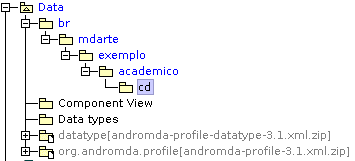
\includegraphics[width=250pt,height=100pt]{imgs/tutorial-mdarte-0000.png}
		\end{figure}
	\item Clique com o botão direito do mouse no pacote “cd” e selecione a opção New Diagram .
Em seguida, selecione Class Diagram.
		
		\begin{figure}[!htb]
			\centering
			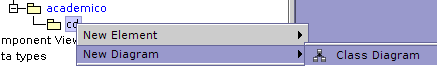
\includegraphics[width=400pt,height=60pt]{imgs/tutorial-mdarte-0001.png}
		\end{figure}
	
	\item Indique o nome desejado para diagrama (ex: Entidades).
	
	\item No diagrama de classe, crie uma nova classe. Clique com o botão direto
	sobre a classe e selecione a opção Specification. Defina o nome da classe como “Estudante”.
	
	\item Crie os atributos na classe Estudante (matricula, nome) selecionando a aba Attributes e
clicando no botão Add. A figura abaixo exemplifica a criação do atributo matricula. O
campo Visibility deve ser public. Não é necessário modelar o atributo id, pois
ele é gerado automaticamente.
		\begin{figure}[!htb]
			\centering
			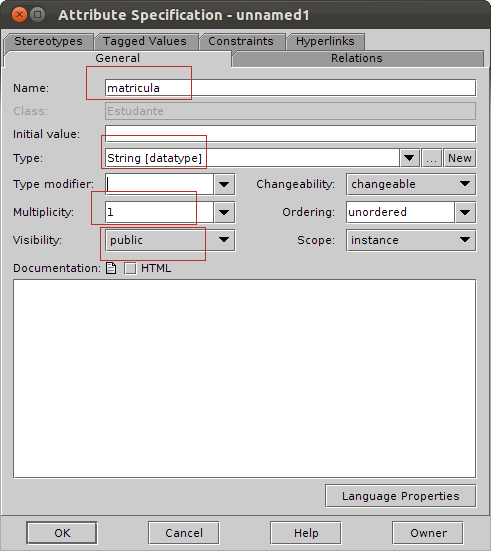
\includegraphics[width=350pt,height=400pt]{imgs/tutorial-mdarte-0002.png}
		\end{figure}
		
	A multiplicidade com valor 1 (campo Multiplicity) indica que o atributo é obrigatório (NOT
NULL), já o valor 0..1 indica que o atributo não é obrigatório. Por padrão, todos os atributos são
gerados como NOT NULL.

	\item Coloque o estereótipo «Unique» no atributo matricula para indicar que cada código deve
ser único, ou seja, não pode haver duas matrículas iguais. Abra a especificação do atributo
matricula e selecione a aba Stereotypes. Nessa aba selecione o estereótipo «Unique».
		\begin{figure}[!htb]
			\centering
			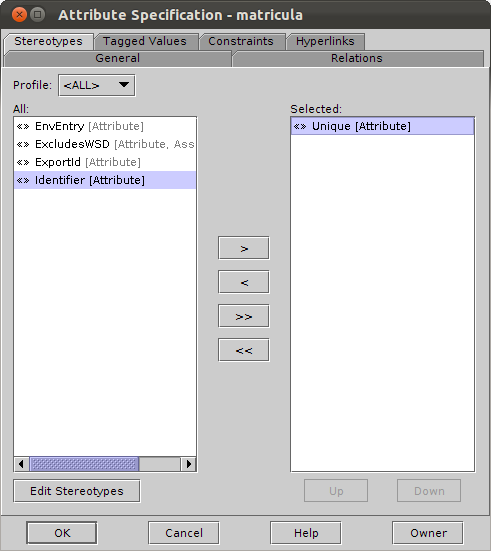
\includegraphics[width=350pt,height=400pt]{imgs/tutorial-mdarte-0003.png}
		\end{figure}
	
	\item Coloque os estereótipos «Entity» e «Manageable» na classe Estudante.
		\begin{figure}[!htb]
			\centering
			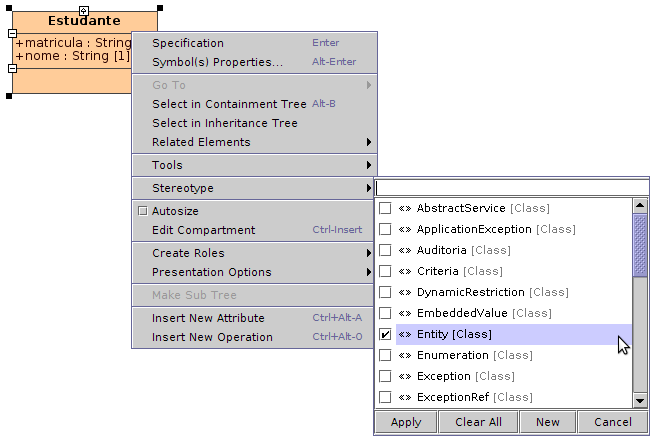
\includegraphics[width=400pt,height=300pt]{imgs/tutorial-mdarte-0004.png}
		\end{figure}
	
	Para cada entidade, também podem ser atribuídos valores etiquetados para
	agregar ao modelo parâmetros para a geração de código. Por exemplo, o valor
	etiquetado @andromda.persistence.table reflete o nome da tabela a ser criada no
	Banco de Dados. Da mesma forma, podemos atribuir estereótipos e valores
	etiquetados aos atributos. Entre os estereótipos temos: «Identifier» que
	determina que o atributo será o identificador do objeto (possível chave
	primária) e «Entity» que determina que o valor do atributo deverá ser único.
	Como exemplo de valores etiquetados temos @andromda.persistence.column que
	define o nome da coluna a ser criada no Banco de Dados e
	@andromda.persistence.column.lenght que define o tamanho da coluna.

	\item No mesmo diagrama de classes, crie outra classe. Clique com o botão
	direto sobre a classe e selecione a opção Specification. Defina o nome da
	classe como “Curso”.
	
	\item Crie os atributos na classe Curso (codigo, nome) selecionando a  aba
	Attributes e clicando no botão Add. O campo Visibility deve ser public, assim
	como feito anteriormente.

	\item Coloque o estereótipo «Unique» no atributo codigo para indicar que cada
	código deve ser único. Abra a especificação do atributo codigo e selecione a
	aba Stereotypes. Nessa aba selecione o estereótipo «Unique».
	
	\item Coloque o estereótipo «Entity» na classe.
	
	\item Agora, crie uma associação entre as classes. Vá no diagrama de classes e
	puxe uma relação Association de uma classe para outra.
	
	\item A associação será de 1 para muitos. Assim, clique duas vezes na
	associação e irá aparecer a tela de especificação. Edite os campos Multiplicity
	definindo valor “0..*” para a entidade Estudante e “1” para a entidade Curso.
		\begin{figure}[!htb]
			\centering
			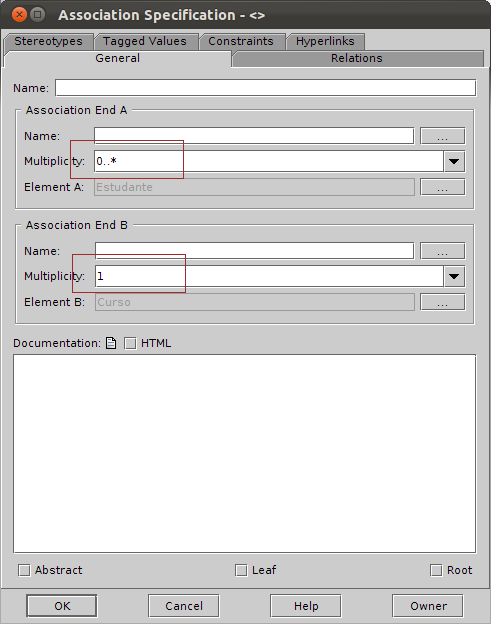
\includegraphics[width=350pt,height=400pt]{imgs/tutorial-mdarte-0005.png}
		\end{figure}
	
	\item A associação deve ser dupla, tanto Estudante quanto Curso devem ser
	visíveis. Dessa forma, mantenha a checkbox Navigable marcada na associação para
	as duas classes. Para isso, clique no botão “...” (reticências) da tela
	anterior.
		\begin{figure}[!htb]
			\centering
			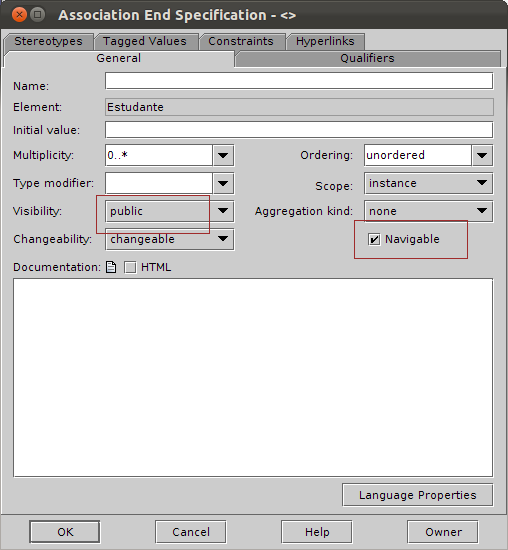
\includegraphics[width=350pt,height=400pt]{imgs/tutorial-mdarte-0006.png}
		\end{figure}
		
	O resultado final será:
		\begin{figure}[!htb]
			\centering
			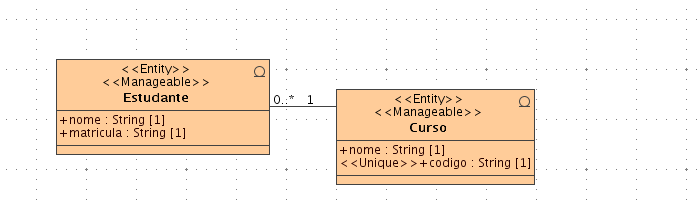
\includegraphics[width=500pt,height=200pt]{imgs/tutorial-mdarte-0007.png}
		\end{figure}
	
	\item No diretório da aplicação, execute o comando maven para validar o modelo
	e gerar o script SQL de criação do Banco de Dados. O resultado apresentado deve
	ser “BUILD SUCCESFULL”.

\end{enumerate}
\chapter{Desenvolvendo o primeiro projeto com o MDArte}

Neste capítulo iremos construir um projeto básico usando o MDArte. O projeto
consistirá de um sistema web simples para administrar um ambiente acadêmico,
onde poderemos cadastrar cursos e gerenciar suas informações, bem como inserir
alunos, inscrevê-los nos e gerenciar suas informações.

\section{Criação de um Novo Projeto}

O plugin do MDArte para o \texttt{Maven} já possui um procedimento parametrizado
para criação de projetos, que funciona como um \texttt{wizard}, onde o usuário
deve responder a perguntas. Através das respostas fornecidas, o MDArte
direcionará a criação da estrutura básica e dos artefatos básicos de
configuração de projetos. O procedimento para criação de um novo projeto é:

\begin{enumerate}
\item Abra o terminal (\texttt{command prompt}) e vá para o diretório onde se
deseja criar o projeto. O projeto será gerado em um subdiretório do
diretório escolhido com o mesmo nome da pasta definido na geração do projeto.

\item Digite o comando: \texttt{maven andromdapp:generate}

\item As perguntas devem ser respondidas de acordo com o projeto a ser
desenvolvido. Abaixo as respostas adequadas para o exemplo desenvolvido neste
capítulo (perguntas em negrito):

\textbf{Please enter your first and last name (i.e. Rodrigo Salvador):} \\
MDArte\\
\textbf{Please enter the name of your J2EE project (i.e. Sistema Academico):}\\
Sistema Academico\\
\textbf{Please enter the id for your J2EE project (i.e. sistemaacademico):}\\
sistemaacademico\\
\textbf{Please enter a version for your project (i.e. 1.0):}\\
1.0\\
\textbf{Please enter the base package name for your J2EE project (i.e. br.mdarte.exemplo.academico):}\\
br.mdarte.exemplo.academico\\
\textbf{Would you like to enable security? (enter 'yes' or 'no')?}\\
yes\\
\textbf{Would you like to use oAuth (enter 'yes' or 'no') ?}\\
no\\
\textbf{Would you like to use MDArte's default Controle Acesso (enter 'yes' or
'no') ?}\\
yes\\
\textbf{Would you like to use modules (enter 'yes' or 'no')?}\\
yes\\
\textbf{Please enter the EJB version number (enter '2' or '3'):}\\
3\\
\textbf{Please enter the Struts version number (enter '1' or '2'):}\\
2\\
\textbf{Would you like to enable the JUnit support for general testing? (enter
'yes' or 'no')? }\\
 no\\
\textbf{Please enter the database backend for the persistence layer: (enter
'hypersonic' or 'mysql' or 'oracle' or 'postgres')}\\
 postgres\\
 
\item Após receber as respostas, o MDArte criará um subdiretório onde será
gerada a estrutura inicial do projeto. A partir desse momento chamaremos esse
diretório de \texttt{<DiretorioProjeto>}.

\item Ainda no console, vá para o diretório onde está seu projeto:
\texttt{<DiretorioProjeto>}.

\item Digite \texttt{maven}. Isto obrigará o \texttt{Maven} a obter todos os
artefatos (por exemplo, bibliotecas) de que o projeto dependerá.

\end{enumerate}

\section{Controle de Acesso}

Neste tutorial estaremos utilizando funcionalidades de controle de acesso, porém
não é nosso propósito explorar suas funcionalidades. Assim, estaremos utilizando
um projeto de controle de acesso desenvolvido pela comunidade do MDArte.

O projeto pode ser obtido a partir do repositório \texttt{Git} do MDArte, pelo
endereço \texttt{https://github.com/MDArte/controleacesso.git}. Por fim, edite
também o arquivo \texttt{project.properties} do \texttt{ControleAcesso} para
configurar o tipo de Banco de Dados a ser utilziado, conforme realizado com o
projeto SistemaAcademico. Note que a propriedade \texttt{dataSource.name} está
definida como \texttt{controleacessoDS}.

Novamente, precisaremos criar um arquivo de configuração do Banco de Dados,
localizado no diretório
\texttt{\textdollar{}JBOSS\_HOME/server/default/deploy/}. O nome do arquivo deve
seguir a mesma formatação mencionada, terminando em \texttt{-ds.xml} (ex.:
\texttt{aplicacoes-ds.xml}), podendo estar no mesmo arquivo com as configurações
do projeto SistemaAcademico.

Exemplo:

\begin{framed}
	\lstinputlisting[language=xml]{files/ControleAcesso-ds.xml}
\end{framed}

Note que no exemplo anterior o ControleAcesso estará utilizando a mesma base de
dados do projeto SistemaAcademico, definida pela tag \texttt{<connection-url>}.
Agora, execute os seguinte comandos, na raiz do projeto \texttt{ControleAcesso},
para gerar, compilar e copiar os pacotes para o diretório
\texttt{\textdollar{}JBOSS\_HOMEHOME/server/default/deploy/}:

\begin{framed}
	\lstinputlisting[language=bash]{files/compila-ca}
\end{framed}

\section{Modelando o nosso primeiro projeto}

Vamos começar agora a modelar o nosso exemplo, mostrando o quão rápido e simples
pode ser usar o MDArte e todo o seu poder de geração.

Para esta parte do tutorial usaremos o \texttt{MagicDraw}. Na barra de
ferramentas do \texttt{MagicDraw}, clicaremos em \texttt{Open Project} e
abriremos o xml do projeto, \texttt{SistemaAcademico.xml} no caminho
\texttt{<DiretorioProjeto>/mda/src/uml/}.

\subsection{Modelando a camada de domínio}
Na camada de domínio, estarão as classes do domínio da aplicação. Elas serão
entidades e estarão associadas a algum modo de persistência. Afim de
contornar os problemas provenientes da utilização de bancos de dados relacionais
em conjunto com o paradigma de orientação à objeto, o MDArte usa o \texttt{framework}
\texttt{Hibernate}\footnote{\hypertarget{http://hibernate.org/orm/}{http://hibernate.org/orm/}}
para gerenciar esta camada.

As classes da camada de domínio deverão conter o estereótipo \texttt{«Entity»} e
os atributos que serão persistidos. Todas as classes de entidade devem
obrigatoriamente estar no pacote \texttt{<PacoteProjeto>.cd}, em que
\texttt{<PacoteProjeto>} é o pacote definido para o projeto.

Neste exemplo, especificamente, iremos também marcar nossas entidades com o
estereótipo \texttt{«Manageable»}, tal marcação diz para o MDArte que desejamos
que seja gerado um \texttt{CRUD} padrão para tais entidades, sem a necessidade de
modelarmos o mesmo diretamente.

\begin{enumerate}
\item Crie a mesma estrutura de pacotes que foi definida na criação do projeto.
Dentro da estrutura, crie o pacote “cd”. Podemos ver o resultado na imagem
~\ref{cria_estrutura_pacotes}. 
\begin{figure}[H]
	\centering
	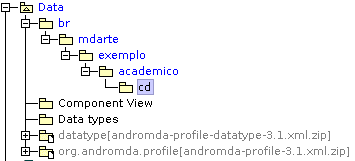
\includegraphics[width=250pt,height=100pt]{imgs/tutorial-mdarte-0000.png}
	\caption{Criação da estrutura de pacotes do projeto e do pacote cd.}
	\label{cria_estrutura_pacotes}
\end{figure}
\item Clique com o botão direito do mouse no pacote “cd” e selecione a opção
\texttt{New Diagram} .Em seguida, selecione \texttt{Class Diagram}. Como mostra
a Figura \ref{cria_diagrama_classe}.
\begin{figure}[H]
	\centering
	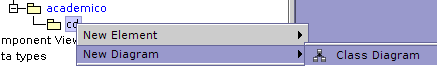
\includegraphics[width=400pt,height=60pt]{imgs/tutorial-mdarte-0001.png}
	\caption{Criação do diagrama de classes da camada de domínio.}
	\label{cria_diagrama_classe}
\end{figure}
	
\item Indique o nome desejado para o diagrama (ex: Entidades).
	
\item No diagrama de classe, crie uma nova classe. Clique com o botão direto
sobre a classe e selecione a opção \texttt{Specification}. Defina o nome da
classe como \texttt{“Estudante”}.
	
\item Crie os atributos na classe Estudante (matricula, nome) selecionando a aba
\texttt{Attributes} e clicando no botão \texttt{Add}. A figura abaixo
exemplifica a criação do atributo matricula. O campo \texttt{Visibility} deve
ser \texttt{public}. Não é necessário modelar o atributo \texttt{id}, pois ele é
gerado automaticamente. Como mostra a Figura \ref{config_parametro}.

\begin{figure}[H]
	\centering
	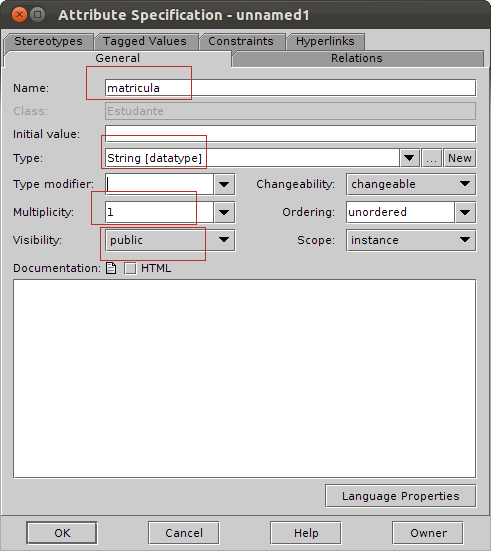
\includegraphics[width=350pt,height=400pt]{imgs/tutorial-mdarte-0002.png}
	\caption{Configuração do parâmetro matrícula da classe Estudante.}
	\label{config_parametro}
\end{figure}
		
A multiplicidade com valor 1 (campo \texttt{Multiplicity}) indica que o atributo é
obrigatório (\texttt{NOT NULL} ), já o valor \texttt{0..1} indica que o atributo
não é obrigatório. Por padrão, todos os atributos são gerados como \texttt{NOT
NULL}.

\item Coloque o estereótipo \texttt{«Unique»} no atributo \texttt{matricula}
para indicar que cada código deve ser único, ou seja, não pode haver duas
matrículas iguais. Abra a especificação do atributo \texttt{matricula} e
selecione a aba \texttt{Stereotypes}. Nessa aba selecione o estereótipo
\texttt{«Unique»}, como na figura \ref{add_estereotipo_matricula}.

\begin{figure}[H]
	\centering
	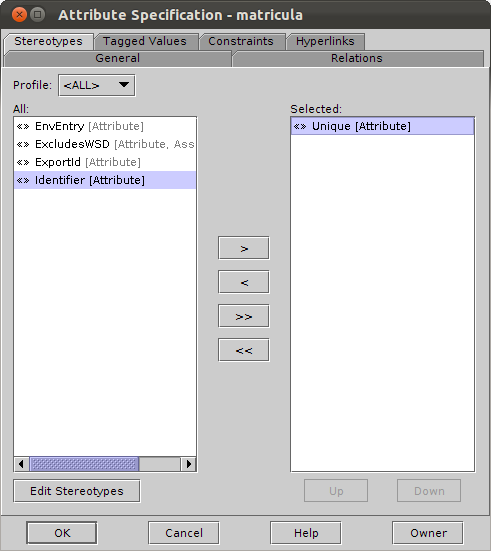
\includegraphics[width=350pt,height=400pt]{imgs/tutorial-mdarte-0003.png}
	\caption{Adição de estereótipo no atributo matrícula.}
	\label{add_estereotipo_matricula}
\end{figure}
	
\item Coloque os estereótipos \texttt{«Entity»} e \texttt{«Manageable»} na
classe \texttt{Estudante}, como na figura \ref{add_estereotipo_estudante}. 
\begin{figure}[H]
	\centering
	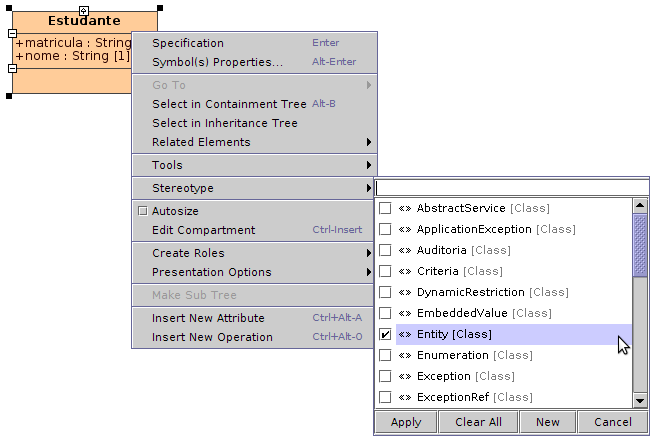
\includegraphics[width=400pt,height=300pt]{imgs/tutorial-mdarte-0004.png}
	\caption{Adição dos estereótipos Entiti e Manageable na classe estudante.}
	\label{add_estereotipo_estudante}
\end{figure}
	
\item No mesmo diagrama de classes, crie outra classe. Clique com o botão direto
sobre a classe e selecione a opção \texttt{Specification}. Defina o nome da classe como
\texttt{“Curso”}.
	
\item Crie os atributos na classe \texttt{Curso} (\texttt{codigo},
\texttt{nome}) selecionando a aba \texttt{Attributes} e clicando no botão
\texttt{Add}. O campo \texttt{Visibility} deve ser \texttt{public}, assim como
feito anteriormente.

\item Coloque o estereótipo \texttt{«Unique»} no atributo codigo para indicar
que cada código deve ser único. Abra a especificação do atributo codigo e
selecione a aba \texttt{Stereotypes}. Nessa aba selecione o estereótipo
\texttt{«Unique»}.
	
\item Coloque o estereótipo \texttt{«Entity»} na classe.
	
\item Agora, crie uma associação entre as classes. Vá no diagrama de classes e
puxe uma relação \texttt{Association} de uma classe para outra.
	
\item A associação será de \texttt{1 para muitos}. Assim, clique duas vezes na associação
e irá aparecer a tela de especificação. Edite os campos \texttt{Multiplicity} definindo
valor “0..*” para a entidade \texttt{Estudante} e “1” para a entidade
\texttt{Curso}, como na figura ~\ref{define_multiplicidade_associacao}.
\begin{figure}[H]
	\centering
	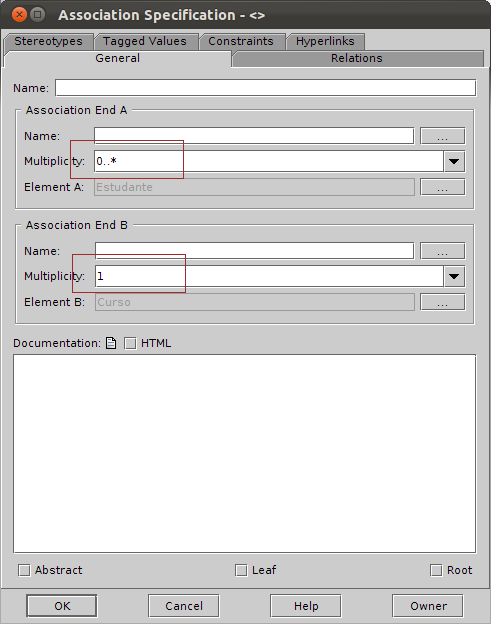
\includegraphics[width=350pt,height=400pt]{imgs/tutorial-mdarte-0005.png}
	\caption{Definindo multiplicidade da associação.}
	\label{define_multiplicidade_associacao}
\end{figure}
	
\item A associação deve ser dupla, tanto \texttt{Estudant} e quanto
\texttt{Curso} devem ser visíveis. Dessa forma, mantenha a \texttt{checkbox}
\texttt{Navigable} marcada na associação para as duas classes. Para isso, clique
no botão “...” (reticências) da tela anterior, como na imagem
~\ref{config_navigable_associacao}.
\begin{figure}[H]
	\centering
	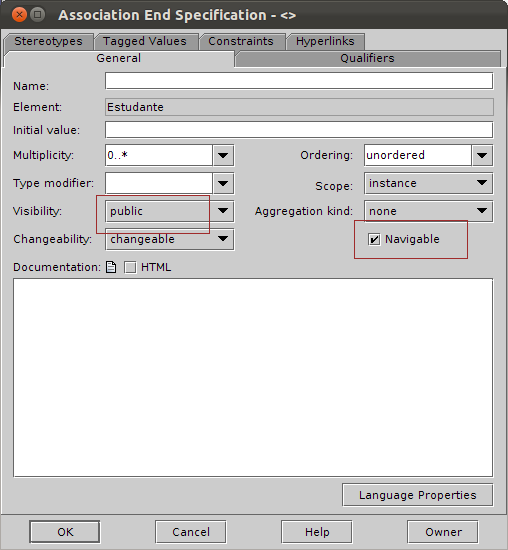
\includegraphics[width=350pt,height=400pt]{imgs/tutorial-mdarte-0006.png}
	\caption{Configuração da navegabilidade da associação.}
	\label{config_navigable_associacao}
\end{figure}
		
O resultado final pode ser visto na imagem ~\ref{resultado_diagrama_classe}: \hfill

\begin{figure}[H]
	\centering
	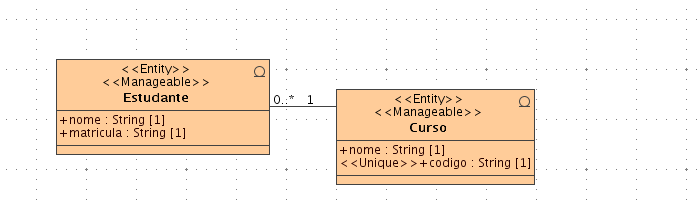
\includegraphics[width=500pt,height=200pt]{imgs/tutorial-mdarte-0007.png}
	\caption{Resultado final da modelagem da camada de domínio.}
	\label{resultado_diagrama_classe}
\end{figure}
	
\item No diretório da aplicação, execute o comando maven para validar o modelo e
gerar o script \texttt{SQL} de criação do Banco de Dados. O resultado
apresentado deve ser \texttt{“BUILD SUCCESFULL”}.
	
\item Observe que dois novos arquivos \texttt{xml} terão sido criados no caminho
\texttt{<DiretorioProjeto>/mda/src/uml/} com os nomes
\texttt{sistemaacademico-geral-Curso.xml} e
\texttt{sistemaacademico-geral-Estudante.xml} , com os crud \texttt{default}
gerados pelo MDArte. Agora precisamos importar os casos de uso criados pelo
MDArte para o \texttt{xml} geral do nosso projeto
(\texttt{SistemaAcademico.xml}). Para isso iremos na barra de ferramentas do
\texttt{MagicDraw} clicaremos em \texttt{file} e na lista de opções que se
abrirá clicaremos em \texttt{import}. Na janela que se abrirá selecionaremos os
modelos que queremos adicionar e clicaremos em \texttt{open}, como na imagem 
~\ref{importa_modulo_geral}:
 \begin{figure}[H]
	\centering
	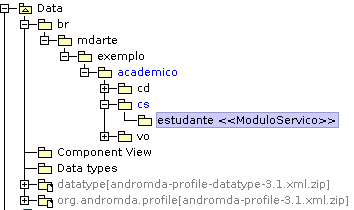
\includegraphics[width=200pt,height=200pt]{imgs/tutorial-mdarte-0008.png}
	\caption{Criação do pacote para a camada de serviço.}
	\label{importa_modulo_geral}
\end{figure} 

O resultado da importação na nossa estrutura de diretórios pode ser visto na
imagem \ref{resultado_arvore_diretórios}.
\begin{figure}[H]
	\centering
	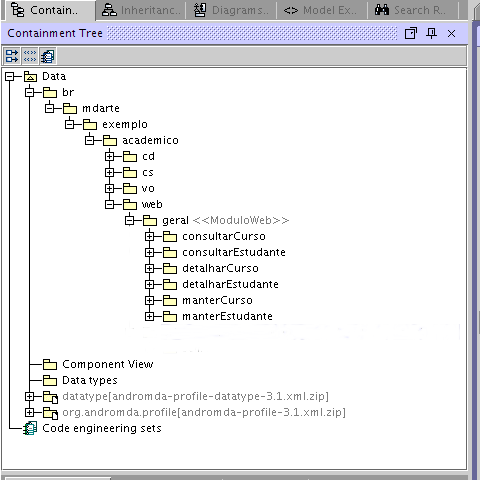
\includegraphics[width=200pt,height=200pt]{imgs/tutorial-mdarte-0019.png}
	\caption{Arvore de diretórios do projeto após a importação dos CRUDS gerados
	automaticamente.}
	\label{resultado_arvore_diretórios}
\end{figure} 

Agora precisamos regerar o projeto, bem como os módulos separados, para isso,
executaremos então os comandos:
	
\begin{framed}
	\lstinputlisting[language=bash]{files/compila-cruds}
\end{framed}

\end{enumerate}

\subsection{Criando o Banco de Dados}

Durante a execução do comando \texttt{maven}, todas as classes são criadas
automaticamente. Além disso, também é gerado o código \texttt{SQL} de criação de
tabelas do Banco de Dados. O script \texttt{SQL} pode ser encontrado em
\texttt{<DiretorioProjeto>/core/cd/target/schema-create.sql}. Abrindo o arquivo
é possível notar a presença de comandos de crição das tabelas \texttt{ESTUDANTE}
e \texttt{CURSO}.

Execute o conteúdo do arquivo no Banco de Dados utilizado.

Como exemplificação dos casos de usos que serão elaborados por este documento,
execute o seguinte script \texttt{SQL} para criar a base inicial. Note que o
script foi escrito para PostgreSQL e deve ser adaptado para o Banco de Dados
escolhido.

\begin{framed}
	\lstinputlisting[language=sql]{files/exemplo.sql}
\end{framed}

\subsection{Modelando a camada de serviços}

Na camada de serviço serão implementadas as classes responsáveis pela lógica de
negócio da aplicação. As classes especificadas se tornarão os serviços
(\texttt{API}) da aplicação. Os serviços definidos no modelo se tornarão
disponíveis através de \texttt{Session Beans}.

Os \texttt{Session Beans} são componentes de negócio. A lógica de negócio dos
componentes \texttt{EJB} se encontram nestes componentes. Existem dois tipos de
Componentes \texttt{Session Bean}, o \texttt{Stateless Session Bean} e o
\texttt{Stateful Session Beans}. O \texttt{Stateless} é um componente de negócio
que não mantém conversação com o usuário, não há garantia que chamadas
sucessivas de métodos remotos vão ser feitas no mesmo objeto. O
\texttt{Stateful} é um componente que mantêm estado, com ele temos a garantia
que chamadas sucessivas de métodos remotos feitas por um mesmo cliente serão
processadas por um mesmo objeto.

Os \texttt{beans} \texttt{EJB} precisam ser modelados em um diagrama de classes.
As classes destes beans precisam ter o estereótipo \texttt{«Service»}. Todas as
classes de serviço devem estar no pacote \texttt{<PacoteProjeto>.cs}, em que
\texttt{<PacoteProjeto>} é o pacote definido para o projeto.

\begin{enumerate}
\item Crie um pacote \texttt{<PacoteProjeto>.cs.estudante}. Clique então com o
botão direito sobre a pasta estudante, na opção \texttt{Stereotype}, selecione o
estereótipo \texttt{«ModuloServico»} e clique em \texttt{Apply}. O resultado
pode ser visto na imagem ~\ref{cria_pacote_servico}:
 \begin{figure}[H]
	\centering
	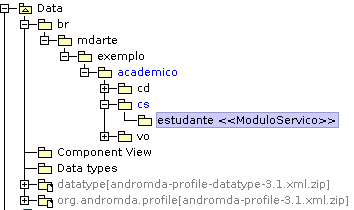
\includegraphics[width=200pt,height=200pt]{imgs/tutorial-mdarte-0008.png}
	\caption{Criação do pacote para a camada de serviço.}
	\label{cria_pacote_servico}
\end{figure} 
	
\item Crie um diagrama de classe dentro do pacote \texttt{estudante}, com o nome
que desejar.
	
\item Crie uma classe com nome \texttt{EstudanteHandler} e estereótipo
\texttt{«Service»}.A classe \texttt{EstudanteHandler} deve ficar como na figura
\ref{cria_sevico_estudante}.
\begin{figure}[H]
	\centering
	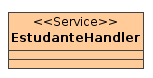
\includegraphics[width=150pt,height=120pt]{imgs/tutorial-mdarte-0009.png}
	\caption{Criação da classe de serviço EstudanteHandler.}
	\label{cria_sevico_estudante}
\end{figure} 
	
\item Crie uma classe com nome \texttt{EstudanteException} e estereótipo
\texttt{«ApplicationException»}, como na imagem ~\ref{cria_estudante_exception}.
\begin{figure}[H]
	\centering
	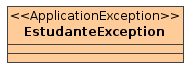
\includegraphics[width=150pt,height=120pt]{imgs/tutorial-mdarte-0010.png}
	\caption{Criação da classe estudante exception.}
	\label{cria_estudante_exception}
\end{figure}
	
\item Arraste para o diagrama de classes recém criado no pacote estudante a
classe \texttt{Estudante}.
	
\item Crie uma relação de dependência entre as classes \texttt{EstudanteHandler}
e \texttt{Estudante}, assim como entre \texttt{EstudanteHandler} e
\texttt{EstudanteException}. Para isso, utilize a opção do \texttt{MagicDraw}
ilustrada na figura abaixo. Clique na opção, depois clique na classe, ou método,
de origem e arraste a seta até a classe destino, como na imagem
\ref{cria_dependencia_servico}.

\begin{figure}[H]
	\centering
	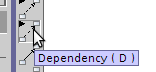
\includegraphics[width=110pt,height=90pt]{imgs/tutorial-mdarte-0012.png}
	\caption{Criação da dependência entre as classes do serviço.}
	\label{cria_dependencia_servico}
\end{figure}

\item Verifique se o diagrama está como a figura
\ref{resultado_diagrama_classe_servico}.
\begin{figure}[H]
	\centering
	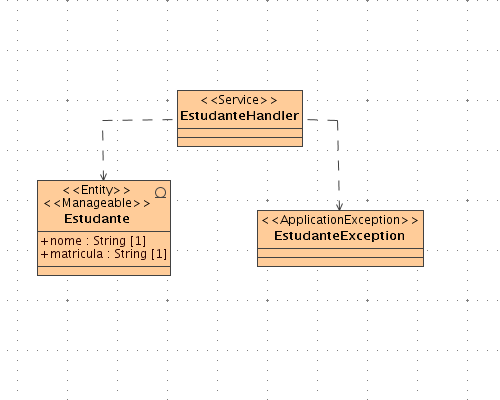
\includegraphics[width=300pt,height=350pt]{imgs/tutorial-mdarte-0011.png}
	\caption{Diagrama de classe completo do módulo de serviço para a classe
	Estudante.}
	\label{resultado_diagrama_classe_servico}
\end{figure}

\item A dependência entre \texttt{EstudanteHandler} e
\texttt{EstudanteException} fará com que todos os métodos de
\texttt{EstudanteHandler} possam lançar a exceção \texttt{EstudanteException}.
Se a dependência tivesse sido entre algum método de \texttt{EstudanteHandler} e
não com a própria classe, somente o método com dependência poderia lançar a
exceção.

A dependência entre \texttt{EstudanteHandler} e \texttt{Estudante} cria os
métodos de acesso ao banco na classe de serviço.

\item Agora faça o mesmo para criar um modulo de serviço para a classe Estudante.
	
\item No diretório da aplicação, execute o comando maven para validar o modelo e
gerar as classes de serviço. O resultado apresentado deve ser \texttt{“BUILD
SUCCESSFULL”}.
\end{enumerate}

\section{Implementando as classes de controle dos cruds gerados}

Nessa seção vamos implementar as classes de controle dos casos de uso gerados.
Para isso, abriremos os arquivos \texttt{<nomeCasoDeUso>ControleImpl}.java.
Esses arquivos são pontos de implementação onde deve ser concentrado todo o
código que se queira adicionar manualmente às classes de controle. Como tais
arquivos só são gerados caso ainda não existam, o código colocado neles não será
sobrescrito, ao contrario do que ocorre se inserirmos manualmente codigo nos
arquivos \texttt{<nomeCasoDeUso>Controle.java}.

De acordo com os casos de uso gerados automaticamente pelo gerador de cruds do
MDArte, iremos implementar respectivamente os seguintes código nos seguintes
arquivos, que devem portanto ser abertos no \texttt{Eclipse} ou em outra
\texttt{IDE} desejada:

\begin{enumerate}
\item ConsultaEstudanteControleImpl.java :
\begin{framed}
	\lstinputlisting[language=java]{files/ConsultaEstudanteControleImpl.java}
\end{framed}
		
\item MantemEstudanteControleImpl.java :
\begin{framed}
	\lstinputlisting[language=java]{files/MantemEstudanteControleImpl.java}
\end{framed}

\item DetalhaEstudanteControleImpl.java:
\begin{framed}
	\lstinputlisting[language=java]{files/DetalhaEstudanteControleImpl.java}
\end{framed}

\item ConsultaCursoControleImpl.java :
\begin{framed}
	\lstinputlisting[language=java]{files/ConsultaCursoControleImpl.java}
\end{framed}

\item MantemCursoControleImpl.java :
\begin{framed}
	\lstinputlisting[language=java]{files/MantemCursoControleImpl.java}
\end{framed}

\item DetalhaCursoControleImpl.java :
\begin{framed}
	\lstinputlisting[language=java]{files/DetalhaCursoControleImpl.java}
\end{framed}

\end{enumerate}

Agora, no terminal, no <DiretorioProjeto> executaremos o seguinte comando :

\begin{framed}
	\lstinputlisting[language=bash]{files/compile-deploy}
\end{framed}

Abriremos agora o eclipse, daremos \texttt{Start} no servidor \texttt{Jboss} e
verificaremos então no navegador o resultado do nosso sistema. Para dar
\texttt{Start} no servidor iremos na aba \texttt{Servers} no nossa \texttt{IDE},
selecionaremos o servidor e clicaremos então no botão de \texttt{Start} (Verde),
como na imagem \ref{server_start}:
\begin{figure}[H]
	\centering
	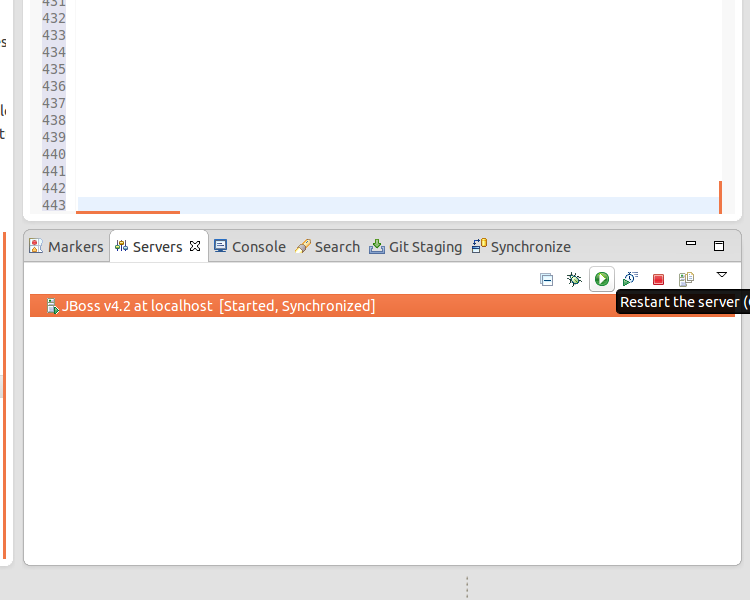
\includegraphics[width=400pt,height=250pt]{imgs/tutorial-mdarte-0015.png}
	\caption{Inicializando o servidor JBoss.}
	\label{server_start}
\end{figure}

Para acessar o sistema, abriremos o navegador e acessaremos a url
\texttt{http://localhost:8080/sistemaacademico/}. Primeiramente será aberta a
página de login do sistema, como na imagem \ref{pagina_login}:
\begin{figure}[H]
	\centering
	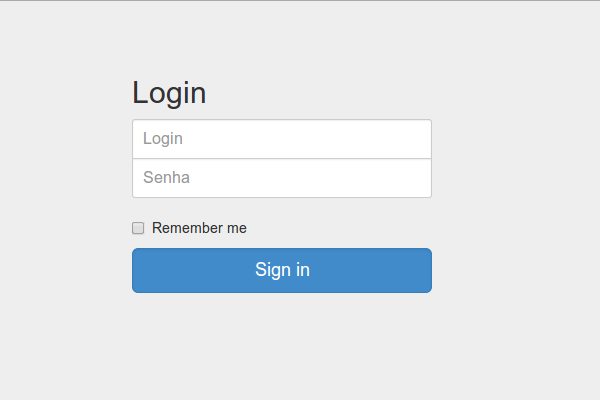
\includegraphics[width=300pt,height=250pt]{imgs/tutorial-mdarte-0013.png}
	\caption{Página de login do Sistema Acadêmico.}
	\label{pagina_login}
\end{figure}

Feito o login, a tela inicial do sistema será aberta como na imagem
\ref{pagina_inicial}.
\begin{figure}[H]
	\centering
	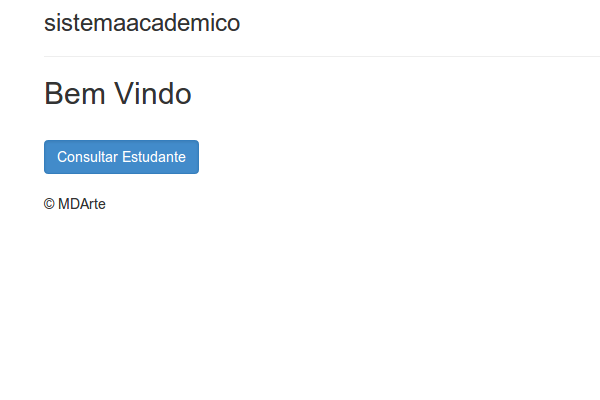
\includegraphics[width=300pt,height=250pt]{imgs/tutorial-mdarte-0017.png}
	\caption{Página incial do Sistema Acadêmico.}
	\label{pagina_inicial}
\end{figure}

Ao clicar no botão \texttt{Consulta Estudante} seremos redirecionados para a
página de consulta no caso de uso de mesmo nome como na imagem
\ref{pagina_consulta_estudante}.
\begin{figure}[H]
	\centering
	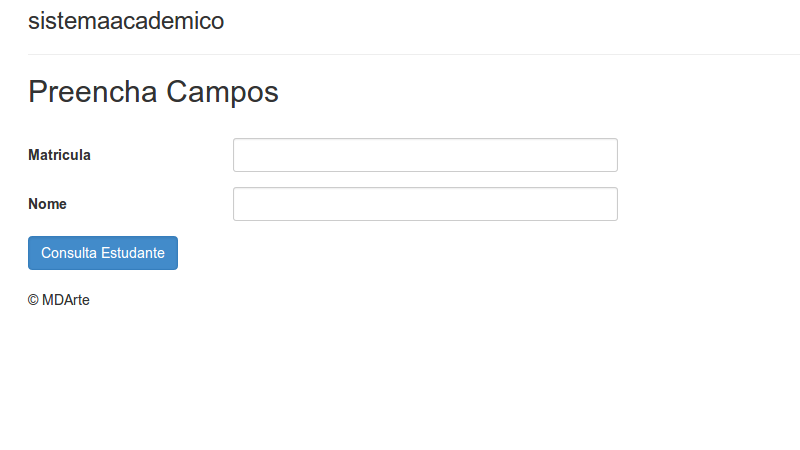
\includegraphics[width=300pt,height=250pt]{imgs/tutorial-mdarte-0018.png}
	\caption{Página incial de Consulta Estudante.}
	\label{pagina_consulta_estudante}
\end{figure}

Se pesquisarmos sem nenhum filtro veremos uma lista completa dos estudantes
registrados como na imagem \ref{resultado_busca_sem_filtro}.
\begin{figure}[H]
	\centering
	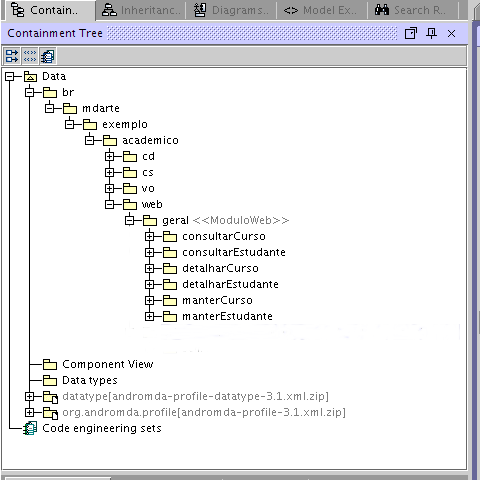
\includegraphics[width=300pt,height=250pt]{imgs/tutorial-mdarte-0019.png}
	\caption{Resultado da busca sem filtro pelos estudantes.}
	\label{resultado_busca_sem_filtro}
\end{figure}
\chapter{Funcionalidades do MDArte}

Neste capítulo iremos explorar algumas funcionalidades que já existem no MDArte,
a fim de agilizar e simplificar o processo de desenvolvimento. Para tal
alteraremos os modelos de \texttt{CRUD} gerados automaticamente pelo
\texttt{MDArte}. Para evitar que as alterações feitas sejam sobrescritas por
engano, vá no diagrama de classe que descreve as entidades do Banco de Dados,
abra a especificação da classe \texttt{Estudante}, selecione a aba
\texttt{stereotypes} e remova o estereótipo \texttt{«Manageable»}.

\section{Campo com Autocomplete}

Nesta seção veremos como implementar um \texttt{autocomplete} para um
determinado campo de texto. Iremos transformar o campo \texttt{matricula} do
caso de uso \texttt{Consulta Estudante} em um campo com \texttt{autocomplete}.

O modelo inicial do caso de uso \texttt{Consulta Estudante} no  \texttt{CRUD}
para a entidade estudante pode ser visto na imagem \ref{modelo_consulta_estudante}:

\begin{figure}[H]
	\centering
	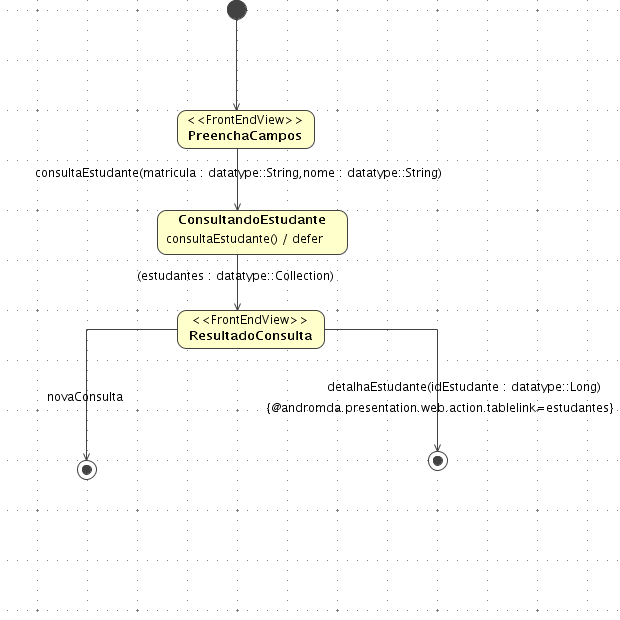
\includegraphics[width=350pt,height=300pt]{files/imgs/tutorial-mdarte-0028.png}
	\caption{Modelo do caso de uso Consulta Estudante.}
	\label{modelo_consulta_estudante}
\end{figure}

Abriremos a especificação da \texttt{transition} que sai da \texttt{front end
view} de nome \texttt{preencha os campos}, clicaremos no botão \texttt{edit}, no
\texttt{fieldset} \texttt{trigger}. Na aba \texttt{parameters}, da janela
\texttt{signal event specification}, que será aberta automaticamente, dê duplo
clique no nome do parâmetro \texttt{matricula} e será então aberta a
especificação do parâmetro. Selecione então a aba \texttt{tagged values},
selecione o \texttt{tagged value}
\texttt{@andromda.presentation.web.view.field.type} e clique no botão
\texttt{create value}. Selecione então a opção \texttt{autocomplete}, como na
imagem \ref{field_type_autocomplete}.

\begin{figure}[H]
	\centering
	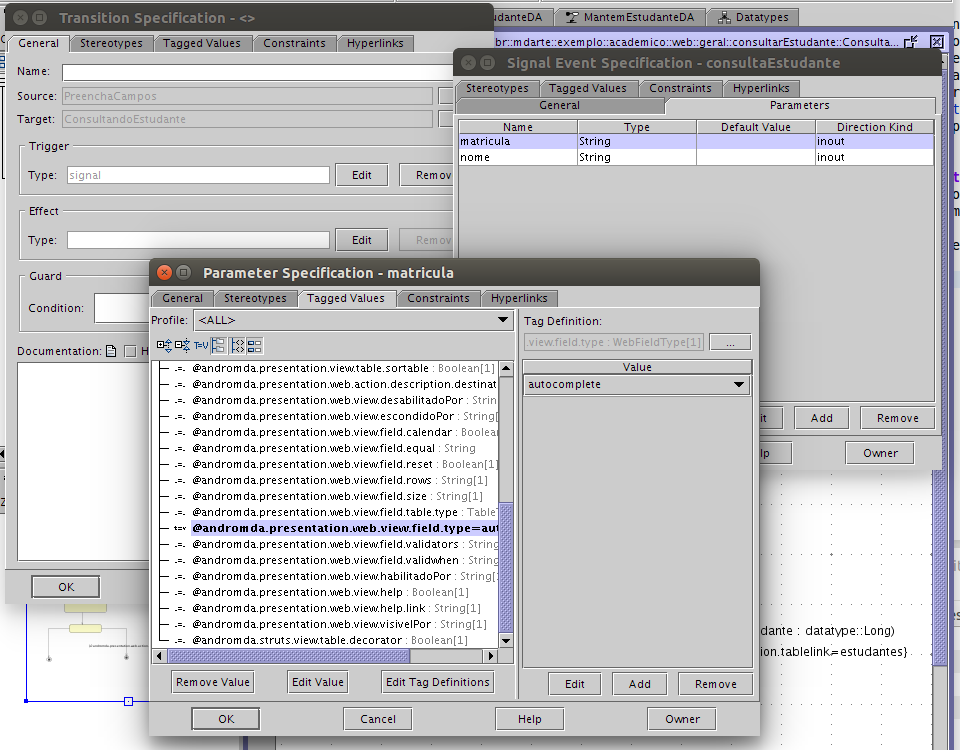
\includegraphics[width=350pt,height=300pt]{files/imgs/tutorial-mdarte-0027.png}
	\caption{Adicionando o field type 'autocomplete' à um campo da view.}
	\label{field_type_autocomplete}
\end{figure}

Agora executaremos o seguinte comando no terminal na raiz do projeto:
\begin{lstlisting}[language=bash]
maven mda -Dprojeto=sistemaacademico-geral-Estudante
\end{lstlisting}

Feito isto, o \texttt{MDArte} gerará automaticamente toda a estrutura
responsável por receber e tratar as requisições assíncronas para o preenchimento do
\texttt{autocomplete}, restando ao desenvolver apenas implementar no
\texttt{ControleImpl} a filtragem dos valores retornados, de acordo com o valor
do campo. Para isto, criaremos, na classe
\texttt{ConsultaEstudanteControleImpl}, um método seguindo o seguinte padrão 
\texttt{protected String[]
<nome-do-campo><nome-do-caso-de-uso>AutoComplete(java.lang.String query,
org.andromda.bpm4struts.ViewContainer container)}. Vejamos abaixo um exemplo de
implementação para o \texttt{autocomplete} do nosso campo de \texttt{matrícula}:

\lstinputlisting[language=java, frame=single, breaklines=true] {files/java/autocomplete.java}

Agora executaremos o seguinte comando para compilar e dar \texttt{deploy} no
\texttt{Sistema Acadêmico} :

\begin{lstlisting}[language=bash, frame=single, breaklines=true]
maven compile deploy
\end{lstlisting}

Feito isto, daremos \texttt{start} no \texttt{JBoss} e abriremos o sistema e
faremos login. Na tela \texttt{Preencha os Campos} do caso de uso
\texttt{Consulta Estudante} podemos agora verificar o \texttt{autocomplete}
funcionando, como na imagem \ref{exemplo_autocomplete}.

\begin{figure}[H]
	\centering
	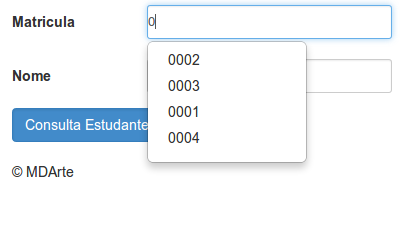
\includegraphics[width=350pt,height=300pt]{files/imgs/tutorial-mdarte-0029.png}
	\caption{Exemplo de autocomplete.}
	\label{exemplo_autocomplete}
\end{figure}
\section{Estratégia de paginação}

Estratégias de paginação foram criadas para comportar diferentes tipos de tabela
e paginação. Nas versões anteriores, a paginação era feita do mesmo jeito para
as tabelas Struts e Ajax porém elas tinham estruturas diferentes o que gerava
erros nas tabelas. Dessa forma, não poderíamos usar a tabela Ajax pois tinhamos
como prioridade ter a tabela Struts funcionando. Com as estratégias de paginação
podemos utilizar qualquer tipo de tabela sem ter que alterar a estrutura dos
DAOs e damos a opção para o desenvolvedor customizar a paginação do jeito que
quiser.

Nesta seção demonstraremos como utilizar estratégias de paginação. Primeiro,
apresentaremos a classe abstrata \texttt{PaginationStrategy}:

\lstinputlisting[language=java, frame=single, breaklines=true] {files/java/PaginationStrategy.java}

A classe abstrata \texttt{PaginationStrategy} é gerado no pacote util do
projeto. Nele você seta a página a ser obtida,  o número de linhas por
página e o número de páginas a serem retornadas pela \texttt{query} e
\texttt{criteria}.

Nela há a função \texttt{paginateResult} que possui duas assinaturas diferentes.
O desenvolvedor tem que implementar essas funções caso deseje criar a sua
própria estratégia. Um exemplo de implementação de estratégia é o
\texttt{PaginationSimple.java} que é utilizado para a paginação da tabela ajax.

\lstinputlisting[language=java, frame=single, breaklines=true] {files/java/PaginationSimple.java}

Além dessa estratégia, criamos outras duas: \texttt{PaginationDisplaytag} para as tabelas Struts e \texttt{NoPagination} caso não seja preciso de paginação.

A pasta em que sua implementação deve ser criada é
<projeto>/common/src/java/<pacote\_do\_projeto>/util e o import a ser feito é
\texttt{<pacote\_do\_projeto>.util.<nome>}.

Demonstramos um simples exemplo para instanciar uma estratégia abaixo:

\begin{lstlisting}[language=java, frame=single, breaklines=true]
	import br.mdarte.exemplo.academico.util.PaginationDisplaytag;
	import br.mdarte.exemplo.academico.util.Constantes;
	
	Integer pagina = ((Integer)request.getAttribute(Constantes.PARAMETRO_PAGINA)); //Struts 1
	Collection exemplos = ServiceLocator.instance().getExemploHandlerBI().recuperaExemplos(new PaginationDisplaytag(paginacao));
\end{lstlisting}
\section{Internacionalização}

Internacionalizar aplicações web é cada vez mais uma tarefa corriqueira de todo
desenvolvedor web e é um dos processos importantes para o aumento da
acessibilidade do sistema. O framework deve permitir mecanismo para facilitar a
utilização de diversas línguas. Para tal, foi construido um conjunto de
ferramentas para facilitar esse processo. A maioria dos frameworks web tem a sua
maneira particular de prover esse mecanismo, mas o que muita gente desconhece é
que existe uma forma padrão de fazer isso,  definida na especificação do Java EE, através da JSP Standard TagLibs.

O MDArte utiliza esse mecanismo e já provê ela configurada. Assim, a
especificação de novas linguas se torna uma tarefa ainda mais fácil.

Segue abaixo os passos para a definições de novas linguas.

\subsection{Mensagens}

Cada arquivo properties conterá todas as traduções do sistema. Todos os textos
do sistemas serão representados por uma \texttt{key}. Cada \texttt{key} e sua
respectiva mensagem, ou seja, \texttt{label} serão listadas em cada arquivo como
properties. Abaixo segue um exemplo:

\begin{lstlisting}[language=xml, frame=single, breaklines=true]
	label.key=Mensagem
\end{lstlisting}

Todas os recursos modelados no diagrama de atividades serão gerados com uma \texttt{key}.
Caso essa \texttt{key} não esteja no arquivo properties, o sistema utilizará a
\texttt{key} como \texttt{label} contudo sem o ponto.

Cada uma das possibilidades será abordada.

\subsubsection{Título de uma Página}

Todo título de página é gerado com uma key para o desenvolvedor possa definir no
custom-resources. 

\begin{lstlisting}[language=html, frame=single, breaklines=true]
	<tiles:put name="title" type="string">
    	<bean:message key="pagina.exemplo.title"/>
	</tiles:put>
\end{lstlisting}

\subsubsection{Campo ou Botão de uma Página}

Todo campo ou botão é gerado com uma key definida pelo o nome do caso de uso
somado com o nome do campo/botão. Segue abaixo um exemplo.

\begin{lstlisting}[language=html, frame=single, breaklines=true]
	<td class="field">
	<s:set name="__value" value="#session.form.nome"/>
	<div id="divnomeConsultaCursoUC" class="textfield field">
    	<label class="textfieldLabel" for="nome"><bean:message key="consulta.curso.uc.preencha.campos.consulta.curso.param.nome"/></label>
    	<s:textfield id="nomeConsultaCursoUC" name="nome" label="%{getText('consulta.curso.uc.preencha.campos.consulta.curso.param.nome')}" value="%{#session.form.nome}" title="" styleId="consultaCursoNome" />
</div>
\end{lstlisting}

\subsubsection{Exception}

Toda mensagem carregando uma \texttt{exception} também é substituída quando a
\texttt{key} na \texttt{exception} é encontrada no \texttt{custom-resource}.
Segue abaixo um exemplo.

\begin{lstlisting}[language=java, frame=single, breaklines=true]
	throw new Exception("ocorre.erro.esperado");

	throw new Exception("ocorre.erro.nao.esperado", exception);
\end{lstlisting}

Existem algumas funções que não interrompem a execução, mas possui o mesmo
efeito do \texttt{exception}. Segue abaixo um exemplo.

\begin{lstlisting}[language=java, frame=single, breaklines=true]
	saveErrorMessage(request, "informando.erro.key");
	saveWarningMessage(request, "informando.aviso.key");
	saveSuccessMessage(request, "informando.sucesso.key");
\end{lstlisting}

\subsubsection{Passagem de Parâmetros}

Existe a possibilidade de passar parâmetros para a mensagem. Será passando um
\texttt{array} de \texttt{string} e na mensagem existirá marcadores informando
onde será colocado o conteúdo do \texttt{array}.

\textbf{Exemplo:}

\texttt{custom-resources.properties}

\begin{lstlisting}[language=xml, frame=single, breaklines=true]
	label.key=Mensagem com parametro {0}
\end{lstlisting}

\texttt{Código:}

\begin{lstlisting}[language=java, frame=single, breaklines=true]
	String[] parametro = new String[1];
	parametro[0] = "param1";
	saveErrorMessage(request, "label.key", parametro);
\end{lstlisting}

Assim será exibido a seguinte mensagem: \texttt{Mensagem com
parametro param1}

\subsection{Arquivo de Configurações}

Edite o arquivo \textbf{<DiretorioProjeto>}/mda/conf/andromda.xml e na
propriedade \texttt{languages} informe os locales que serão utilizados.

Exemplo:

\begin{lstlisting}[language=xml, frame=single, breaklines=true]
	<property name="languages">pt,en,fr</property>
\end{lstlisting}

Após a geração utilizando essa configuração será criado novos três arquivos: 

\begin{lstlisting}[language=xml, frame=single, breaklines=true]
	custom-resources_en.properties
	custom-resources_pt.properties
	custom-resources_fr.properties
\end{lstlisting}

Além do arquivo já criado no geração da aplicação:

\begin{lstlisting}[language=xml, frame=single, breaklines=true]
	custom-resources.properties
\end{lstlisting}

Automaticamente o sistema irá detectar qual locale do browser que o usuário está
utilizando e utilizará o locale correto. Caso não exista o locale pré-definido,
o sistema utilizará o \texttt{custom-resources} padrão.

O desenvolvedor poderá forçar um locale específico pelo código. Exemplo: 

\begin{lstlisting}[language=java, frame=single, breaklines=true]
	//Recuperando o Locale
	Locale locale = (Locale) request.getSession().getAttribute("org.apache.struts.action.LOCALE");

	//Definindo um Locale
	request.getSession().setAttribute("org.apache.struts.action.LOCALE", new Locale("pt", "BR"));
\end{lstlisting}

\section{Modo de Operação}

Usar modo operação permite que o desenvolvedor mostre campos, botões e outros
artefatos de maneira condicionais no frontend. A idéia básica por trás do modo
de operação é a seguinte:

Se um usuário chegar na página através de um botão A, você exibe tal página sem
certas opções. Se um usuário chegar na mesma tela através de um botão B, você
exibe a mesma página com as opções omitidas no caso anterior. O modo de
operação permite que isso seja feito.

A seguir demonstramos um exemplo:

\subsection{Exemplo}

Dados a entidade USUARIO, onde usuario tem os atributos ( nome, email, sexo ['M'
| 'F'], certificadoDeReservista). Porém para sexo igual a 'F' certificado é null
e para 'M' certificado deve ser diferente de null.

Suponhamos agora que o desenvolver deseje mostrar esse usuário. Porém quando o
usuário for masculino deveremos mostrar o certificado e quando for feminino não
mostraremos. Para isso utilizaremos o modo de operação. 

Primeramente defineremos no campo certificado de reservista o modo de operação
CERTIFICADO. Uma vez definido o campo com o modo de operação, ele aparecerá
somente se for invocado desse modo operação, no nosso caso, CERTIFICADO.

Podemos invocar o modo de operação a partir do fluxo ou do controlador para que
apareça o campo certificado. 

Primeiro, demonstramos como ele será invocado no controlador.

\subsection{Invocando pelo Controlador} 

Para definir o valor que tem que ser invocado para mostrar o campo com modo
operação, fazemos:
 
\begin{enumerate}

\item Abrimos a transição, vamos para trigger e clicamos em edite, vamos na aba
parameters e selecionamos o campo a ser colocado o modo de operação, caso o
campo exista clique em edit, caso não exista o campo clique em add.

\begin{figure}[H]
	\centering
	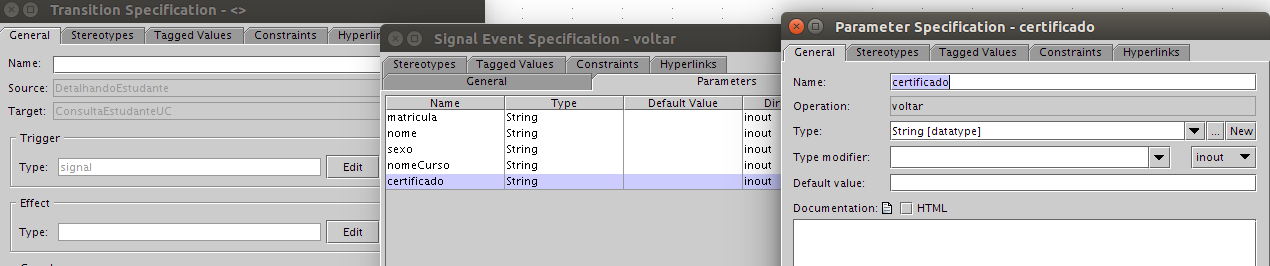
\includegraphics[scale=0.75]{files/imgs/operation-mode-00.png}
	\caption{Criando o campo}
	\label{criando_campo_modo_operacao}
\end{figure}

\item Agora clique na aba Tagged Values:
@andromda.presentation.view.operation.mode.
\item Em seguida clique em Create Value.
\item Agora digite o nova do valor que voce deseja, que no nosso caso será
CERTIFICADO

\begin{figure}[H]
	\centering
	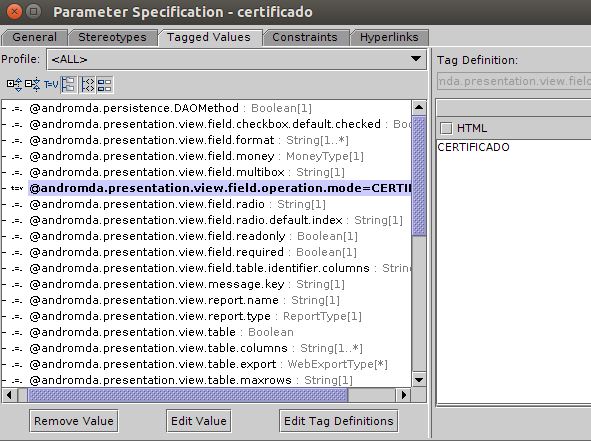
\includegraphics[scale=0.75]{files/imgs/operation-mode-01.png}
	\caption{Adicionando o modo de operação do campo}
	\label{aicionando_modo_operacao_campo}
\end{figure}

\item Pelo Eclipse vá ao ponto de implementação da classe de controle que tem
que disparar o modo de operação e adicione o seguinte código:

\begin{lstlisting}[language=java, frame=single, breaklines=true]
if( estudante.getSexo().getValue().equals("M") ){
	adicionaModoOperacao("CERTIFICADO",container);// <---- Aqui disparamos o MODO OPERACAO
	form.setCertificado(estudante.getCertificado());
}
\end{lstlisting}

\end{enumerate}

Quando chamarmos essa classe de controle, nós iremos invocar o modo de operação
da view caso a condição seja satisfeita nesse caso.

Em seguida, mostraremos como fazer a invocação do modo de operação pelo fluxo.

\subsection{Invocando pelo Fluxo}

Fazendo por fluxo, temos que colocar um valor no valor etiquetado
@andromda.presentation.action.input.operation.mode de uma transição que está
indo para o caso de uso (indo para um estado final) que contém o campo com o
mesmo modo de operação.

\begin{figure}[H]
	\centering
	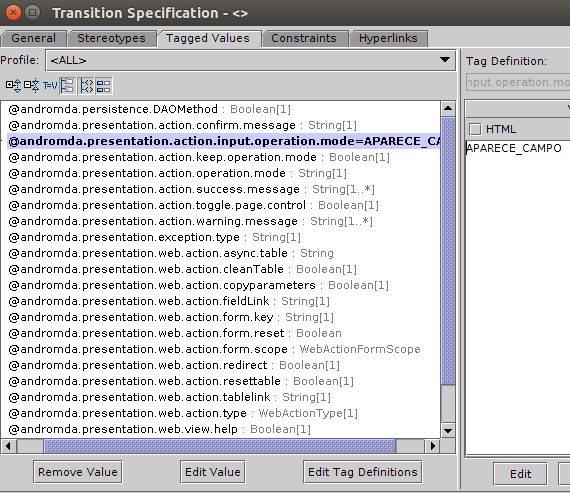
\includegraphics[scale=0.75]{files/imgs/operation-mode-02.png}
	\caption{Adicionando o modo de operação do campo}
	\label{aicionando_modo_operacao_campo}
\end{figure}

Repita o passo 1 da invocação por controlador para ter um campo em que o
funcionamento do modo de operação possa ser testado. Apenas isso precisa ser
feito para fazer modo de operação por fluxo.

Existe um valor no valor etiquetado
@andromda.presentation.action.keep.operation.mode que é também usado em uma
transição que está indo para um estado. Se colocar o valor dele como true você
manterá para o próximo caso de uso o modo de operação recebido de outro caso de
uso.

\subsection{Implementação}

\subsubsection{Sistema}

\subsubsection{Componentes}

\subsection{Na JSP\ldots}

Nas PaginasPersonalizadas, o modo de operação aparece como a tag

<security:containsOperationMode value=“NomeDoModoDeOperacao”>

que envolve o componente definido pelo caso de uso.


\subsection{Regra de ouro do modo de operação}

    Se o componente não possuir nenhum modo de operação definido, ele será
    exibido sempre,  independente se existe ou não um modo de operação definido no sistema.
    
    Se o componente tiver um modo de operação definido,  o componente só será
    exibido na página se o modo de operação do sistema for igual
    
    Você pode definir mais de um modo de operação,  tanto para o sistema quanto
    para um componente. Basta separar os nomes dos modos de operação por vírgula.


\section{Pontos de decisão}

Pontos de decisão são criados quando sua aplicação precisa tomar decisões
dependendo do resultado de uma ação prévia. Utilizamos uma forma de modelagem
ofericida pela especificação UML.

Nela você desenha uma linha de transição a partir da ação conectando-a ao ponto
de decisão. Um ponto de decisão é desenhado como um losango em UML. Já que uma
decisão tem pelo menos dois resultados diferentes, o ponto de decisão terá
múltiplas transições para diferentes ações.

Usaremos como exemplo para introduzir um ponto de decisão o seguinte diagrama de
atividades:

\begin{figure}[H]
	\centering
	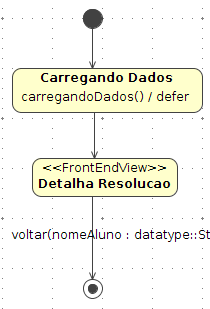
\includegraphics[scale=0.75]{files/imgs/decision-point-00.png}
	\caption{Modelo inicial do exemplo}
	\label{modelo_inicial_ponto_decisao}
\end{figure}

Criamos um ponto de decisão e colocamos uma transição do estado
\textbf{Carregando Dados} para o ponto de decisão:

\begin{figure}[H]
	\centering
	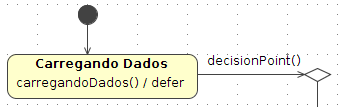
\includegraphics[scale=0.75]{files/imgs/decision-point-01.png}
	\caption{Criando o ponto de decisão}
	\label{criando_ponto_decisao}
\end{figure}

Em seguida na classe de controle do diagrama de atividades criamos uma função
chamada \texttt{decisionPoint}:

\begin{figure}[H]
	\centering
	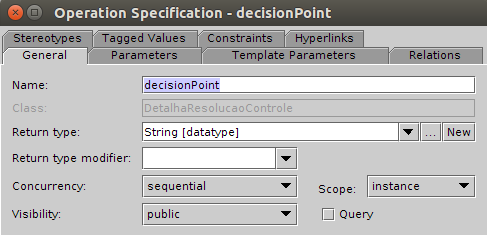
\includegraphics[scale=0.75]{files/imgs/decision-point-02.png}
	\caption{Criando função do ponto de decisão}
	\label{funcao_ponto_decisao}
\end{figure}

Na transição para o ponto de decisão, alteramos a \texttt{trigger} e colocamos o
tipo dela como \texttt{call} e a operação como \texttt{decisionPoint}:

\begin{figure}[H]
	\centering
	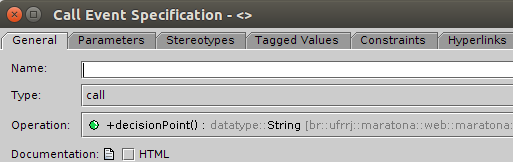
\includegraphics[scale=0.75]{files/imgs/decision-point-03.png}
	\caption{Colocando a função na transição}
	\label{funcao_transicao}
\end{figure}

O próximo passo é passar o início da transição que ia de \textbf{Carregando
Dados} para \textbf{Detalha Resolucao} para o ponto de decisão e criar uma
transição do ponto de decisão para o estado final.

\begin{figure}[H]
	\centering
	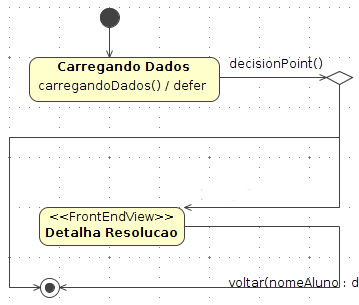
\includegraphics[scale=0.75]{files/imgs/decision-point-04.png}
	\caption{Colocando a função na transição}
	\label{ponto_decisao_com_transicoes}
\end{figure}

Em seguida devemos criar a condição de guarda dessas transições. Na aba
\texttt{General}, clicamos no botão \texttt{Edit} da seção \texttt{Guard}:

\begin{figure}[H]
	\centering
	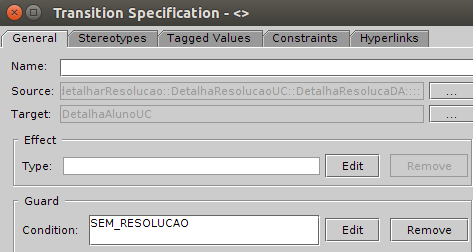
\includegraphics[scale=0.75]{files/imgs/decision-point-05.png}
	\caption{Abrindo a transição}
	\label{abrindo_transição}
\end{figure}

Agora especificamos o nome da condição de guarda e a condição em si. Ambos tem
que ter o mesmo nome:

\begin{figure}[H]
	\centering
	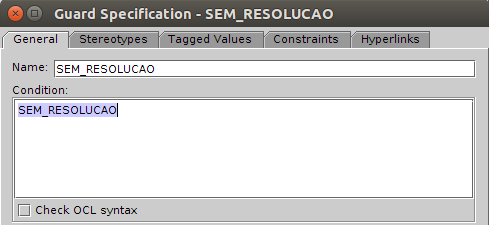
\includegraphics[scale=0.75]{files/imgs/decision-point-06.png}
	\caption{Especificando a condição de guarda}
	\label{condicao_de_guarda}
\end{figure}

Fazemos o mesmo para a outra transição e o modelo final é o seguinte:

\begin{figure}[H]
	\centering
	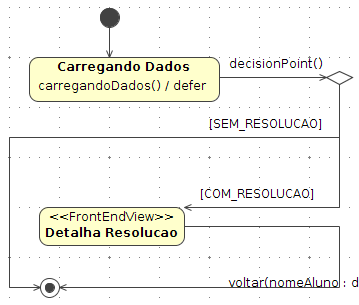
\includegraphics[scale=0.75]{files/imgs/decision-point-07.png}
	\caption{Modelo final}
	\label{modelo_final}
\end{figure}

Agora temos que implementar a função \texttt{decisionPoint}. Ela tem que
retornar uma String que seja uma das condições de guarda especificadas no
modelo. Exemplo de código:

\begin{lstlisting}[language=java, frame=single, breaklines=true]
	public String decisionPoint(DecisionPointForm form, ViewContainer container) throws Exception
	{
		if (form.getIdResolucao() != null) {
			return "COM_RESOLUCAO";
		}
		else {
			return "SEM_RESOLUCAO";
		}
	}
\end{lstlisting}
\section{Tabela assíncrona (JTable)}

Nesta seção veremos como implementar uma tabela \texttt{assíncrona}
(\texttt{JTable}) usando o \texttt{MDArte}. Para tal, vamos considerar como
ponto de partida o modelo do caso de uso \texttt{Consulta Estudante} conforme as
alterações feitas no tópico anterior. Certifique-se de ter removido o
estereótipo \texttt{«Manageable»} da classe \texttt{Estudante} no diagrama de
classes que descreve a \texttt{Camada de domínio}, a fim de evitar que o
\texttt{CRUD} seja re-gerado, sobrescrevendo assim as alterações que faremos.

Veremos agora, por subseções, algumas das funcionalidades disponíveis na tabela
assíncrona.

\subsection{Implementando filtragem assíncrona da tabela}
Nesta seção veremos como criar uma action ajax que reflita nos dados exibidos
por uma tabela ajax. A título de exemplo, faremos uma tela com um formulário e
um botão que, uma vez clicado, recarregará a tabela filtrando-a de acordo com os
dados do formulário. Tomaremos como base a tabela criada no exemplo de criação
de tabelas.

O modelo portanto começará assim:

\begin{figure}[H]
	\centering
	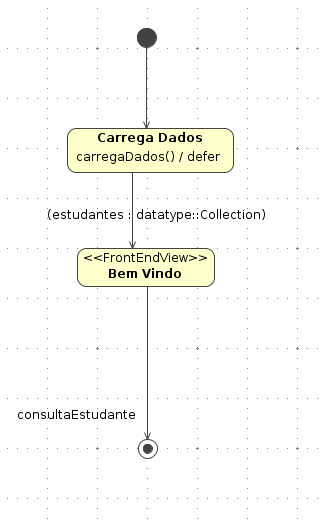
\includegraphics[width=180pt,height=260pt]{files/imgs/tutorial-mdarte-0040.png}
	\caption{Modelagem da filtragem assíncrona da tabela.}
	\label{modelando_filtragem_assincrona}
\end{figure}

Modelaremos então uma \texttt{transition} saindo da \texttt{FrontEndView} que
contém a nossa tabela e retornando para a mesma \texttt{view}, que será
interpretada pelo \texttt{MDArte} como uma ação assíncrona na \texttt{view}.
Abriremos então sua especificação e iremos na aba \texttt{tagged values} e
selecionaremos o \texttt{tagged value}
\texttt{@andromda.presentation.web.action.async.table} e daremos a ele o valor
\texttt{[nome-da-tabela]} (\texttt{estudantes}, nesse caso), esse \texttt{tagged
value} indica qual tabela será afetada pela ação assíncrona, nos permitindo ter
mais de uma de tabela assíncrona na mesma tela, tendo \texttt{actions} que
afetem somente uma tabela sem afetar a outra. Iremos então na aba
\texttt{general} e clicaremos no botão \texttt{edit} no \texttt{fieldset}
\texttt{'trigger'}, daremos o nome que desejarmos o \texttt{trigger} criado, no
exemplo fo idado o nome de \texttt{“filtrar”}, e selecionaremos seu tipo como
\texttt{signal}. Iremos então na aba \texttt{parameters}, ainda na especificação
do \texttt{trigger} e criaremos os parâmetros necessários para o processamento
da requisição, neste exemplo colocaremos só os parâmetros \texttt{matrícula} e
\texttt{nome}, a título de ilustração, e definiremos seus tipos como
\texttt{String}.

O modelo ficará assim:
\begin{figure}[H]
	\centering
	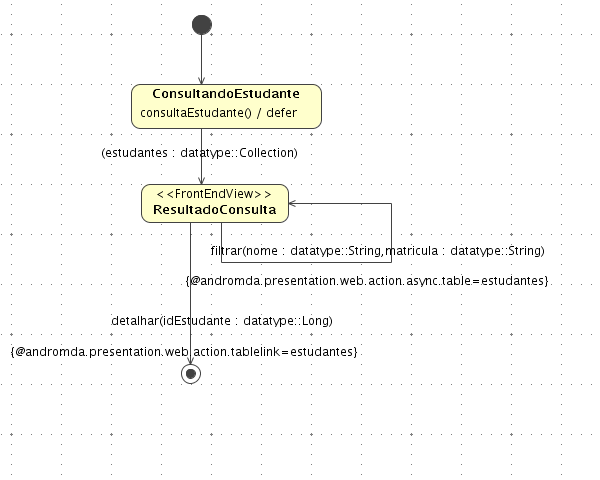
\includegraphics[width=340pt,height=300pt]{files/imgs/tutorial-mdarte-0036.png}
	\caption{Modelagem da filtragem assíncrona da tabela.}
	\label{modelando_filtragem_assincrona}
\end{figure}

Executaremos agora o seguinte comando para validar o modelo e regerar o
sistema:
\begin{lstlisting}[language=bash, frame=single, breaklines=true]
maven mda -Dprojeto=sistemaacademico-geral-Estudante
\end{lstlisting}

Agora adaptaremos, no \texttt{ControleImpl}, os métodos responsáveis pelo
carregamento da tabela, com a assinatura \texttt{public final Collection
load[nome-da-view][nome-da-tabela]Table}, e pelo retorno do número máximo de
elementos na mesma, com a assinatura \texttt{public final Integer
get[nome-da-view][nome-da-tabela]TableLength}, a fim de implementarmos o filtro.
Cada parâmetro da \texttt{trigger} pertencente à \texttt{transition} modelada
será adicionado, em ordem, à lista de parâmetros de cada método, logo antes do
parâmetro \texttt{ViewContainer container}. De acordo com o nosso exemplo, o
código ficará assim:
\lstinputlisting[language=java, frame=single, breaklines=true]{files/java/JTableFiltro.java}

Executaremos agora o seguinte comando para compilar e dar \texttt{deploy} no
sistema:
\begin{lstlisting}[language=bash, frame=single, breaklines=true]
maven compile deploy
\end{lstlisting}

Restartando o servidor e abrindo o caso de uso \texttt{Consulta Estudante},
veremos o resultado do que fizemos:
\begin{figure}[H]
	\centering
	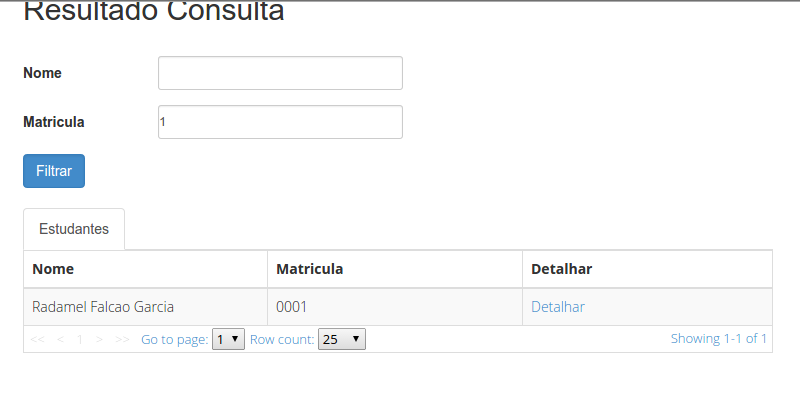
\includegraphics[width=340pt,height=300pt]{files/imgs/tutorial-mdarte-0042.png}
	\caption{Modelagem da filtragem assíncrona da tabela.}
	\label{modelando_filtragem_assincrona}
\end{figure}

\section{Criação de Componente customizado}

Nesta seção veremos como criar um campo customizado em uma tela. Iremos partir
do modelo de \texttt{CRUD} gerado automaticamente pelo \texttt{MDArte}, para a
entidade \texttt{Estudante}, e faremos as alterações necessárias para a criação
de um novo componente. O componente a ser desenvolvido, somente a título de
exemplo, será um campo texto com máscara para \texttt{CPF}.

Podemos ver o estado inicial do modelo na imagem \ref{modelo_consulta_estudante_custom}.

\begin{figure}[H]
	\centering
	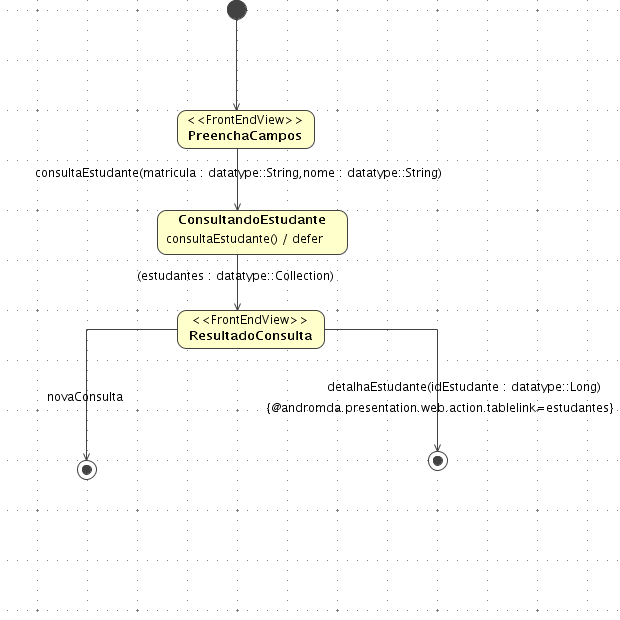
\includegraphics[width=350pt,height=300pt]{files/imgs/tutorial-mdarte-0028.png}
	\caption{Modelo do caso de uso Consulta Estudante.}
	\label{modelo_consulta_estudante_custom}
\end{figure}

Abriremos então a especificação da \texttt{transition}
\texttt{'consultaEstudante'}, clicaremos no botão \texttt{'edit'}, no
\texttt{fieldset} \texttt{'trigger'}, selecionaremos então a aba
\texttt{'parameters'}, da janela aberta quando clicamos o botão anterior, e
clicaremos então no botão \texttt{add}.

Preencheremos então os dados do campo conforme a imagem
\ref{dados_campo_custom_cpf}, SEM, no entanto, clicar no botão \texttt{Ok}.

\begin{figure}[H]
	\centering
	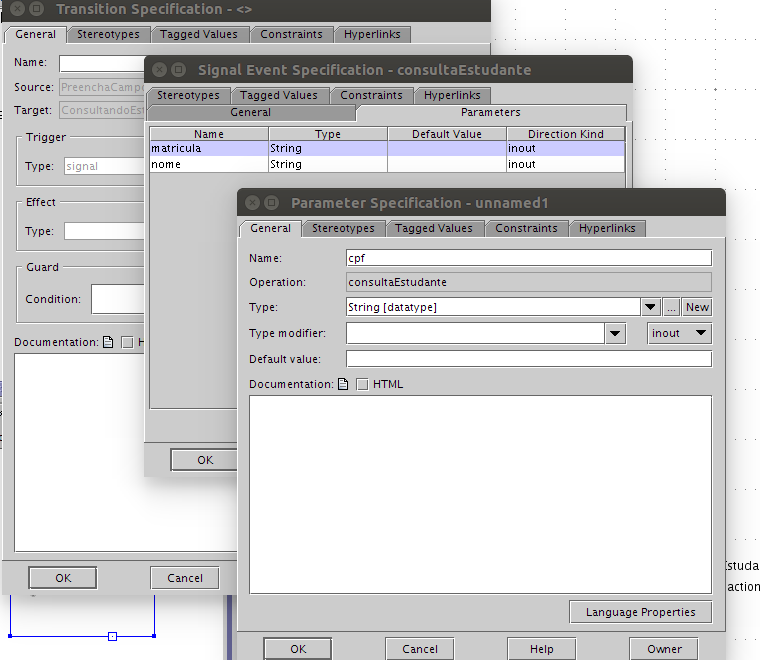
\includegraphics[width=350pt,height=300pt]{files/imgs/tutorial-mdarte-0033.png}
	\caption{Dados do campo 'cpf'.}
	\label{dados_campo_custom_cpf}
\end{figure}

Ainda na mesma janela, selecionaremos a aba \texttt{tagged values},
selecionaremos o \texttt{tagged value} 
\texttt{@andromda.presentation.web.view.field.type}, clicaremos no botão
\texttt{create value} e selecionaremos a opção \texttt{'custom'}, no campo
\texttt{combobox} que será exibido, como na imagem \ref{parametro_cpf_custom}.

\begin{figure}[H]
	\centering
	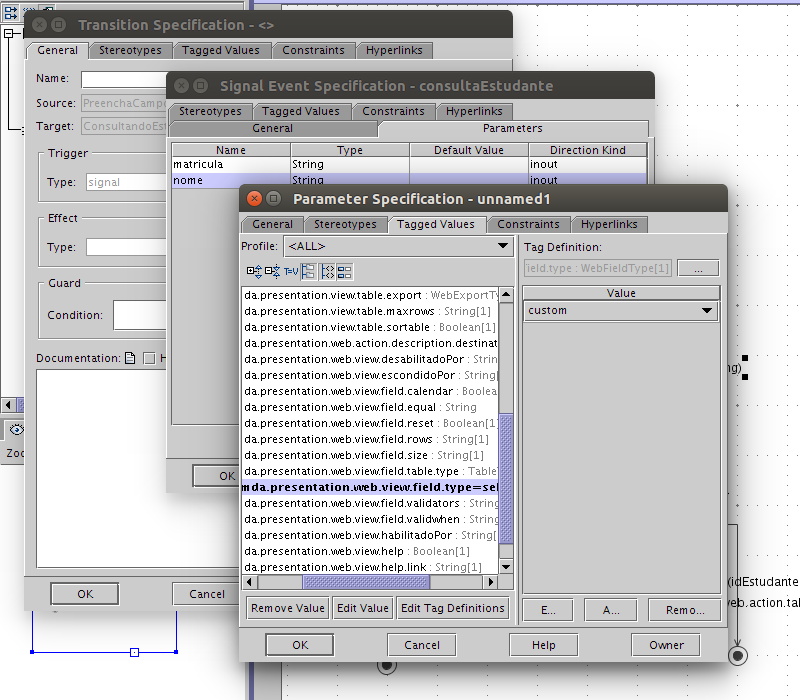
\includegraphics[width=350pt,height=300pt]{files/imgs/tutorial-mdarte-0034.png}
	\caption{Selecionando tipo custom para o campo 'cpf'.}
	\label{parametro_cpf_custom}
\end{figure}

Salvaremos então o modelo e digitaremos os seguintes comandos para regerar o
modelo:

\begin{lstlisting}[language=bash, frame=single, breaklines=true]
maven mda -Dprojeto=sistemaaacademico-geral-Estudante
\end{lstlisting}

Feito isto, o \texttt{MDArte} gerará um arquivo no padrão
\texttt{<nome-do-campo>.jsp}, neste caso, \texttt{cpf.jsp}, no caminho
\texttt{<nome-sistema>/web/<modulo-web>/src/jsp/<caminho-do-pacote-base>/web/<modulo-web>/<nome-caso-de-uso>},
mas você também pode encontrá-lo, no eclipse, através do comando
\texttt{ctrl+shift+r}, digitando o nome do arquivo na janela que é aberta por
esse comando.

Aberto o arquivo, adicionaremos a este o seguinte código \texttt{jsp}:

\lstinputlisting[language=html, frame=single, breaklines=true]{files/jsp/cpf.jsp}

O \texttt{html} adicionado será importado para a tela do sistema no espaço do
formulário dedicado ao campo \texttt{cpf}.

Adicionado o \texttt{jsp} do nosso componente, uma vez que se trata de um campo
de texto com um determinado comportamento (formatar a entrada no modelo do CPF),
precisamos agora adicionar um mecanismo de controle para o comportamento do
campo. Para tal, utilizaremos o \texttt{framework} para \texttt{javascript}
JQuery, uma vez que este já vem com o \texttt{MDArte}, além do fato de o
\texttt{JQuery} já possuir uma funcionalidade nativa que faça isso.

Para adicionar código \texttt{Javascript} manualmente a uma \texttt{view}
precisamos abrir o arquivo \texttt{<nome-da-view>-impl.js}, no mesmo caminho
do arquivo \texttt{jsp} alterado acima. O arquivo alterado é destinado ao código
adicionado pelo desenvolvedor para customizar o comportamento da aplicação, não
sendo sobrescrito durante a geração. Certifique-se, portanto, de estar
adicionando o seu código nestes pontos de implementação, a fim de não perdê-lo
na próxima geração.

Adicionaremos agora o seguinte código \texttt{JavaScript} ao arquivo
\texttt{preencha-campos-impl.js}:

\lstinputlisting[language=c, frame=single, breaklines=true]{files/js/preencha-campos-impl.js}

\appendix
\chapter{Configuração do JBoss e acesso ao banco de dados}
\label{jboss-config}
Neste apêndice veremos como configurar as informações de acesso ao banco de
dados do nosso projeto, bem como demais configurações do nosso servidor de
aplicação (JBoss).

\section{Configuração das propriedades do projeto para acesso ao banco de dados}
Para se configurar o Banco de Dados é necessário modificar o arquivo
\texttt{project.properties} da raiz do projeto, onde se encontram as
propriedades que devem ser alteradas. Os arquivos
\texttt{project.properties} são arquivos onde são definidas propriedades que são
usadas pelo MDArte durante a sua exucação, este, na raiz do projeto,
especificamemte concentra propriedades de acesso ao banco e de deploy(?) do
projeto.

Abaixo estão as propriedades do arquivo de
configuração para cada um dos Bancos de Dados:

\begin{itemize}
	\item [Oracle] \hfill
	\begin{itemize}
		\item dataSource.driver.jar=\textdollar{}\{env.JBOSS\_HOME\}/server/default/lib/ojdbc14.jar
		\item dataSource.driver.class=oracle.jdbc.driver.OracleDriver
		\item sql.mappings=Oracle9i
		\item hibernate.db.dialect=org.hibernate.dialect.Oracle9Dialect
	\end{itemize}
	\item [SQLServer] \hfill
	\begin{itemize}
		\item dataSource.driver.jar=\textdollar{}\{env.JBOSS\_HOME\}/server/default/lib/jtds-1.1.jar
		\item dataSource.driver.class=net.sourceforge.jtds.jdbc.Driver
		\item sql.mappings=MSSQL
		\item hibernate.db.dialect=org.hibernate.dialect.SQLServerDialect
	\end{itemize} 
	\item [Postgres] \hfill
	\begin{itemize}
		\item dataSource.driver.jar=\textdollar{}\{env.JBOSS\_HOME\}/server/default/lib/postgresql.jar
		\item dataSource.driver.class=org.postgresql.Driver
		\item defaultHibernateGeneratorClass=sequence
		\item sql.mappings=PostgreSQL
		\item hibernate.db.dialect=org.hibernate.dialect.PostgreSQLDialect
	\end{itemize}
	\item [MySQL] \hfill
	\begin{itemize}
		\item dataSource.driver.jar=\textdollar{}\{env.JBOSS\_HOME\}/server/default/lib/mysql-connector-java-5.1.6-bin.jar
		\item dataSource.driver.class=com.mysql.jdbc.Driver
		\item defaultHibernateGeneratorClass=native
		\item sql.mappings=MySQL
		\item hibernate.db.dialect=org.hibernate.dialect.MySQLDialect
	\end{itemize}
\end{itemize}

Tais propriedades são as responsáveis por definir qual banco de dados estará
sendo usado no projeto, bem como qual biblioteca será usada para a comunicação
com o banco. Propriedades como a url do banco, nome de usuário, senha etc. não
precisam ser alteradas uma vez que, mais adiante, as definiremos diretamente na
configuração do jboss.

\section{Configuração do JBoss}
Agora veremos como configurar o servidor JBoss e qual a finalidade dos arquivos 
utilizados para tal fim. 

\subsection{Configuração dos datasources utilizados pelo JBoss}
Para a configuração dos datasources utilizados pelo JBoss é preciso criar ou
alterar o arquivo responsável por registrar e gerenciar tais fontes de dados.
O arquivo que deve estar localizado no diretório
\texttt{JBOSS\_HOME/server/default/deploy/}, com formação do nome terminando com
\texttt{-ds.xml} (ex.: \texttt{aplicacoes-ds.xml)}, que deve ter a tag
<local-tx-datasource> preenchida de acordo com as informações  fornecidas no
arquivo \texttt{<projeto>/project.properties}.

Exemplo (usando banco Postgres):

\begin{framed}
	\lstinputlisting[language=xml]{files/sistemaacademico-ds.xml}
\end{framed}

Repare que no exemplo anterior, o nome do Data Source é sistemaacademicoDS, que
deve ser o mesmo nome informado no arquivo \texttt{project.properties} no
diretório raiz do projeto. Aqui também definimos algumas outras propriedades do
datasource sistemaacademicoDS que haviam ficado em aberto antes como a url de
conexão com o servidor de banco de dados, usuario e senha.

\subsection{Configuração do acesso das aplicações ao banco de dados}
Para tal, alteraremos o arquivo \texttt{login-config.xml}, localizado no
diretório \texttt{JBOSS\_HOME/server/default/conf/}. Alteraremos o arquivo
adicionando uma tag \texttt{<application-police name='<nomeAplicacao>'>} com
seus campos devidamente preenchidos como no exemplo abaixo, onde temos a
configuração para o Sistema Acadêmico deste tutorial.

\begin{framed}
	\lstinputlisting[language=xml]{files/sistemaacademico-login-config.xml}
\end{framed}

O arquivo alterado concentra as informações de login para as diversas aplicações
sendo rodadas no servidor, informações como: datasource que contém os dados de
usuário usados no login, query a ser rodada para buscar os dados de usuário,
algoritmo de hash da senha etc. As informações presentes nesse arquivo
permitirão a aplicação do Sistema Acadêmico se conectar a base de dados e validar o usuário no momento de login.


\bibliographystyle{unsrt}
\bibliography{library}

\end{document}

